%!TEX root = Memoria_TFM.tex
\section{Final experiment results}
In this section, the test results obtained from section \ref{sec:Final_archi} are presented as well as the training process.

\subsection{Training and validation process}
The convolutional neural networks has been trained independently for each database as  explained in \ref{sec:Final_archi}. In this section, the training and validation process are detailed for each database.

\subsubsection{CASIA Image database}
In figure \ref{fig:ejecucion2_casia_im_train} the cost and training are represented (\ref{fig:ejecucion2_casia_im_train_cost} and \ref{fig:ejecucion2_casia_im_train_cost} respectively). The training process converges in  low values, smaller than 0.0001; while the validation process converges in a 20\% error from the $250^{th}$ epoch. The iterations, where the training process oscillates sharply, agree with the epochs where the cost oscillates sharply too. After those oscillations, the validation becomes constant and the training error variates in its lowest values.\\
\begin{figure}[htb]
\centering
		\subfigure[Cost at training]{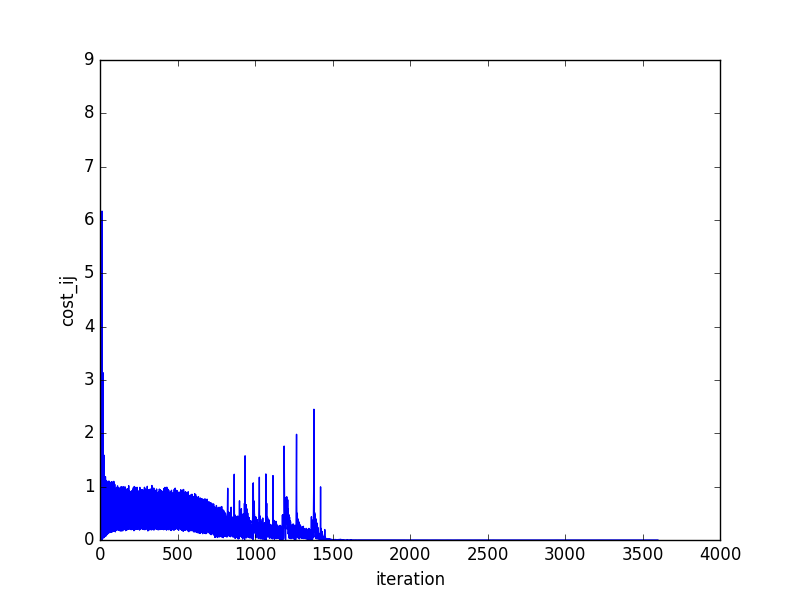
\includegraphics[width=0.47\textwidth]{images/ejecucion2_general/resultados_casia_images/cost.png}\label{fig:ejecucion2_casia_im_train_cost}}
		\subfigure[Error at validation]{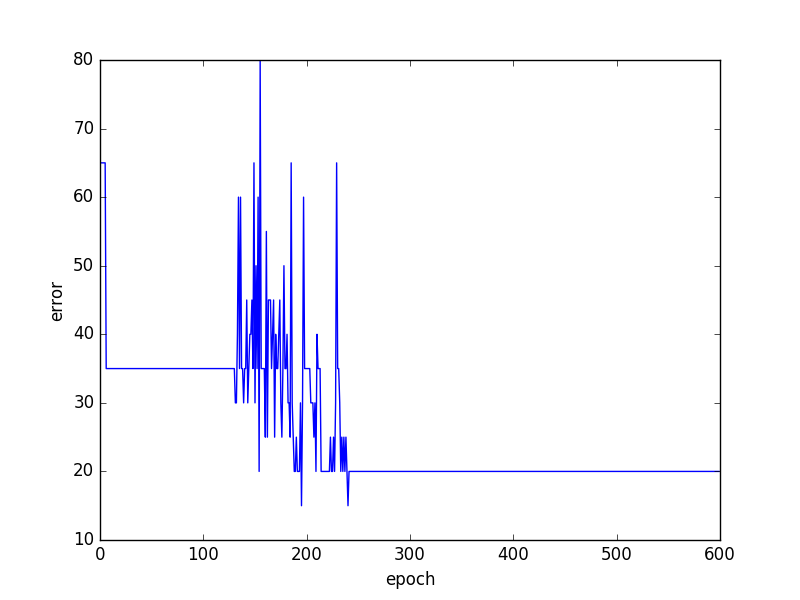
\includegraphics[width=0.47\textwidth]{images/ejecucion2_general/resultados_casia_images/error.png}\label{fig:ejecucion2_casia_im_train_error}}
\caption{Cost (a) and error (b) at training CASIA image database.}
\label{fig:ejecucion2_casia_im_train}
\end{figure}

The saved model to carry out the test performance is the one obtained at iteration 1176 with a 15\% validation error.

\subsubsection{CASIA Video database}
The cost and error obtained at training and validation processes when using the CASIA video database, is represented in figure \ref{fig:ejecucion2_casia_vid_train}. The minimum cost is almost 0 and it is obtained before the $2000^{th}$ iteration, as represented in figure \ref{fig:ejecucion2_casia_vid_train_cost}. The validation converges at the same time as the training, where it oscillates between 7\% and 6\%.\\
\begin{figure}[htb]
\centering
		\subfigure[Cost at training]{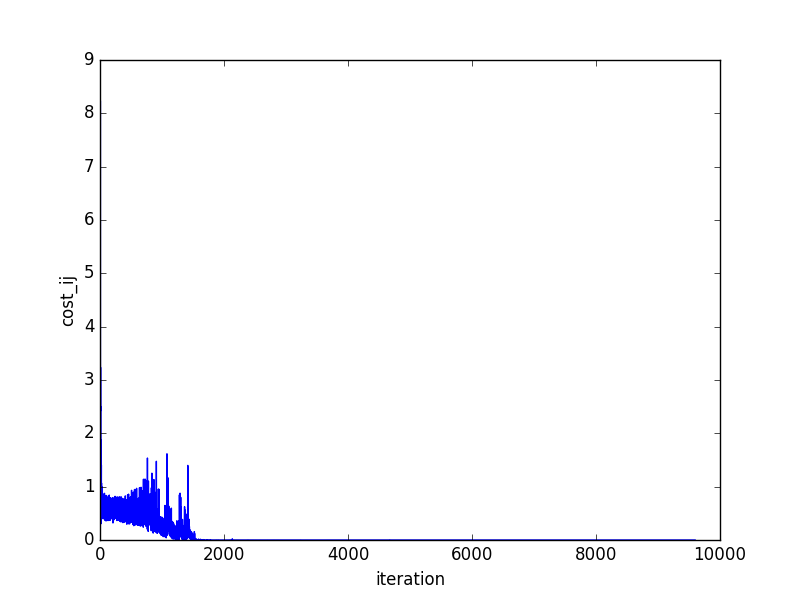
\includegraphics[width=0.47\textwidth]{images/ejecucion2_general/resultados_casia_videos/cost.png}\label{fig:ejecucion2_casia_vid_train_cost}}
		\subfigure[Error at validation]{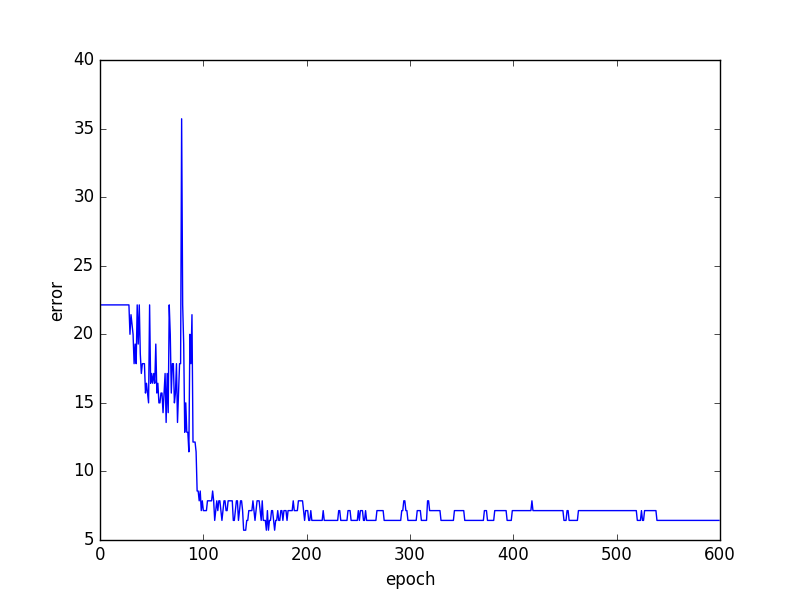
\includegraphics[width=0.47\textwidth]{images/ejecucion2_general/resultados_casia_videos/error.png}\label{fig:ejecucion2_casia_vid_train_error}}
\caption{Cost (a) and error (b) at training CASIA video database.}
\label{fig:ejecucion2_casia_vid_train}
\end{figure}

The best validation performance is obtained at iteration 2240 with a 5.71\% validation error.

\subsubsection{RGB FRAV database}
The cost and error obtained at training and validation processes respectively are represented in figure \ref{fig:ejecucion2_frav_train}. The cost, that can be seen in figure \ref{fig:ejecucion2_frav_train_cost} has a low value when it converges before the 5000th iteration; the cost obtained is $10^{-6}$. The validation error, represented in figure \ref{fig:ejecucion2_frav_train_cost}, fluctuates considerably. The curve should decrease, yet it does not, and in the 200th epoch, the error is constant in 11.25\%. The generalization at validation is not very good and before the 100th epoch the network seems to overfit.\\
\begin{figure}[htb]
\centering
		\subfigure[Cost at training]{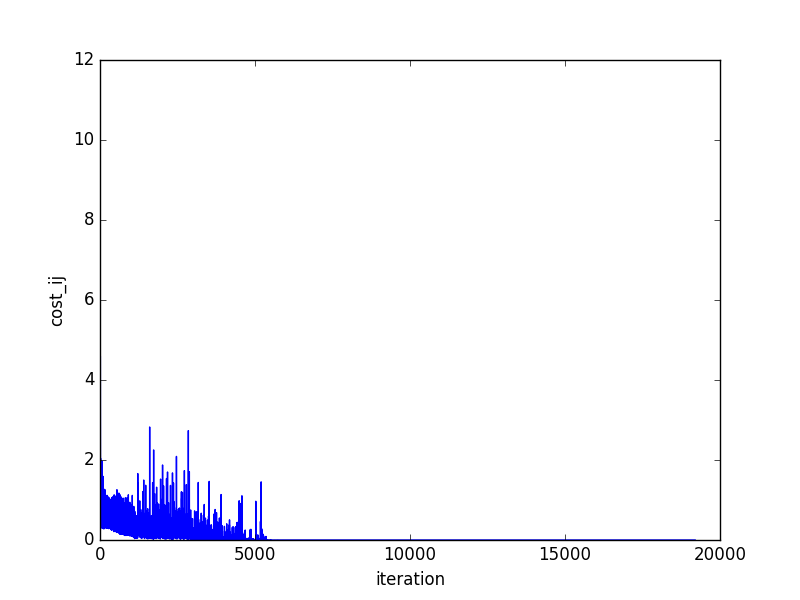
\includegraphics[width=0.47\textwidth]{images/ejecucion2_general/resultados_frav/cost.png}\label{fig:ejecucion2_frav_train_cost}}
		\subfigure[Error at validation]{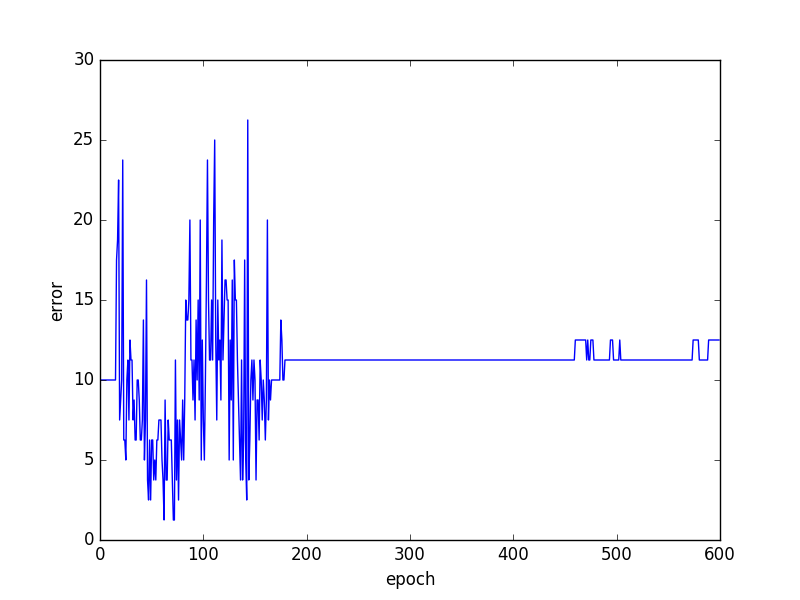
\includegraphics[width=0.47\textwidth]{images/ejecucion2_general/resultados_frav/error.png}\label{fig:ejecucion2_frav_train_error}}
\caption{Cost (a) and error (b) at training RGB FRAV image database.}
\label{fig:ejecucion2_frav_train}
\end{figure}

The best validation score of 1.25\% has been obtained at iteration 2016 which is saved as a model for testing.

\subsubsection{RGB+NIR (feature level) FRAV database}
The RGB+NIR FRAV database, whose images have been added before the training process, has a cost and error which is represented in figure \ref{fig:ejecucion2_frav_feat_train}. The cost at training, that can be seen in \ref{fig:ejecucion2_frav_feat_train_cost} oscillates in the 3500 first iterations until it decreases its value to 0 in the last 100 iterations. The cost at validation oscillates in the same oscillation cost period, where the value gets to 0\% at different times. Subsequently, the value gets to 3,3\%. Although the validation performance does not decrease in a desirable way, it gets a 0\% error which means that the generalization is very good.\\
\begin{figure}[H]
\centering
		\subfigure[Cost at training]{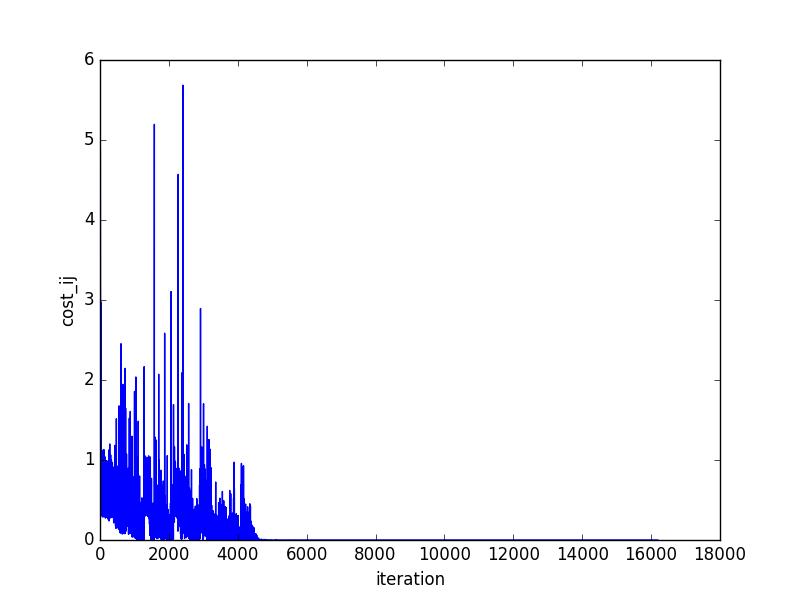
\includegraphics[width=0.47\textwidth]{images/ejecucion2_general/resultados_frav_rgb_nir/cost.png}\label{fig:ejecucion2_frav_feat_train_cost}}
		\subfigure[Error at validation]{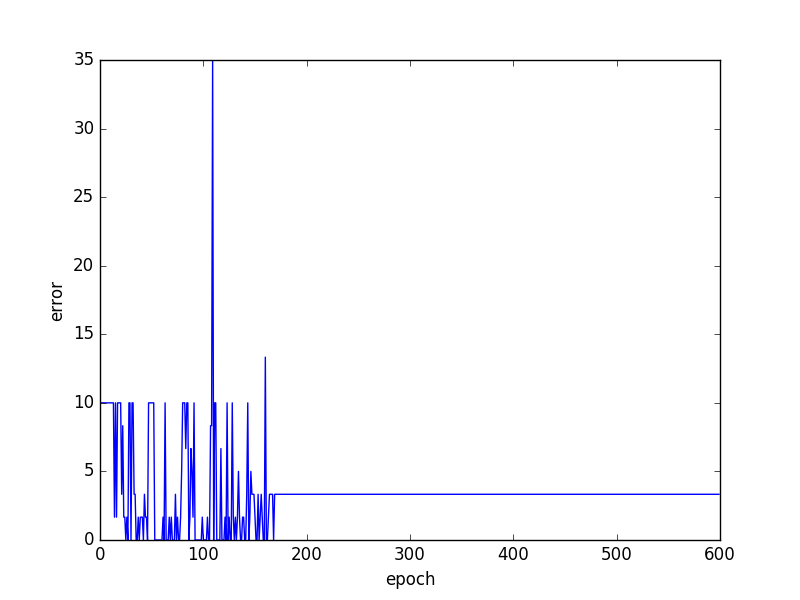
\includegraphics[width=0.47\textwidth]{images/ejecucion2_general/resultados_frav_rgb_nir/error.png}\label{fig:ejecucion2_frav_feat_train_error}}
\caption{Cost (a) and error (b) at training RGB and NIR FRAV (feature level) image database.}
\label{fig:ejecucion2_frav_feat_train}
\end{figure}

The best model is obtained at 702 iteration, when the validation gets 0\% for the first time.

\subsubsection{RGB+NIR (classification level) FRAV database}
In figure \ref{fig:ejecucion2_frav_clas_train} the training cost and the validation error is represented when the database has been trained, first the RGB subset and then NIR subset. These two subsets are trained independently and features of each best model are concatenated to test the performance.\\
\begin{figure}[htb]
\centering
		\subfigure[Cost at training RGB subset]{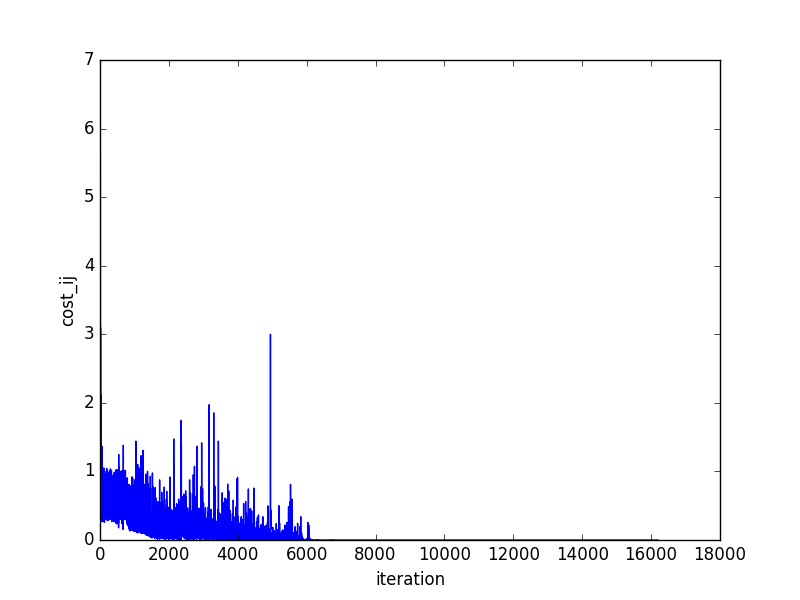
\includegraphics[width=0.47\textwidth]{images/ejecucion2_general/resultados_frav_concatenated/cost_rgb.png}\label{fig:ejecucion2_frav_clas_train_cost_rgb}}
		\subfigure[Error at validation RGB subset]{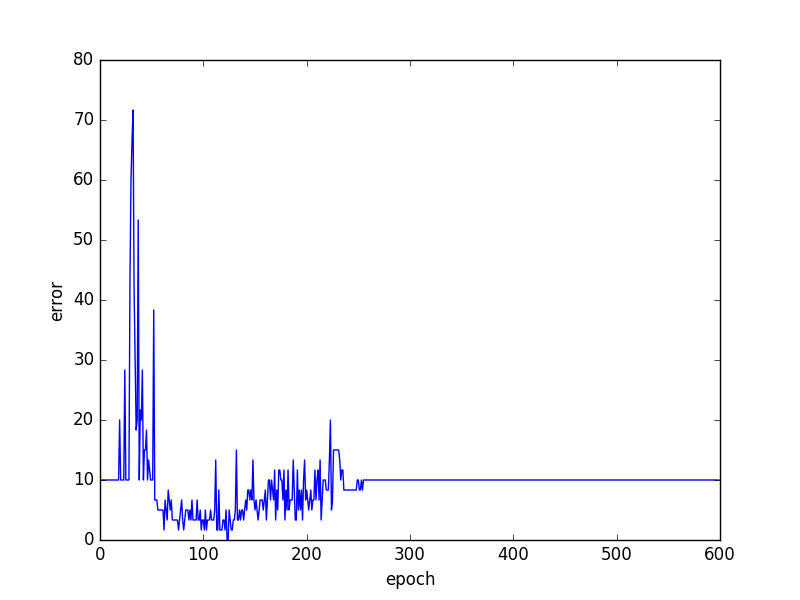
\includegraphics[width=0.47\textwidth]{images/ejecucion2_general/resultados_frav_concatenated/error_rgb.png}\label{fig:ejecucion2_frav_clas_train_error_rgb}}
		\subfigure[Cost at training NIR subset]{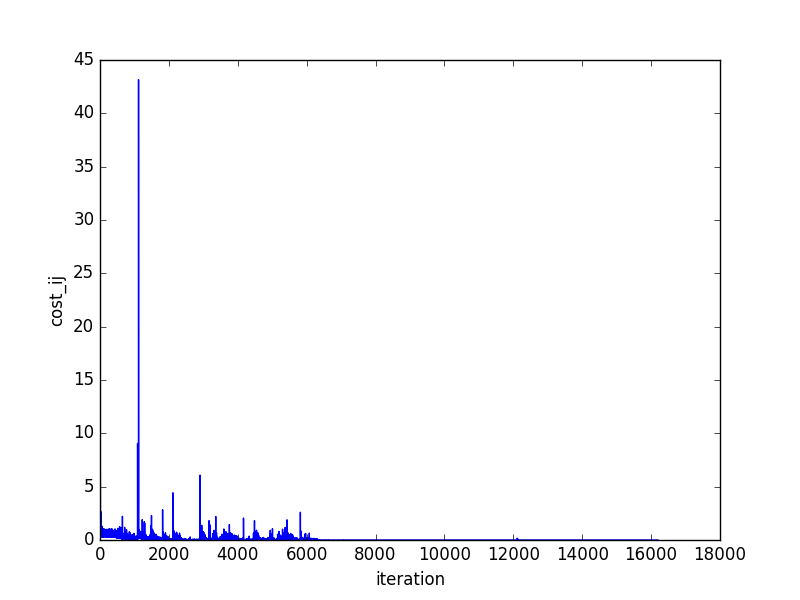
\includegraphics[width=0.47\textwidth]{images/ejecucion2_general/resultados_frav_concatenated/cost_nir.png}\label{fig:ejecucion2_frav_clas_train_cost_nir}}
		\subfigure[Error at validation NIR subset]{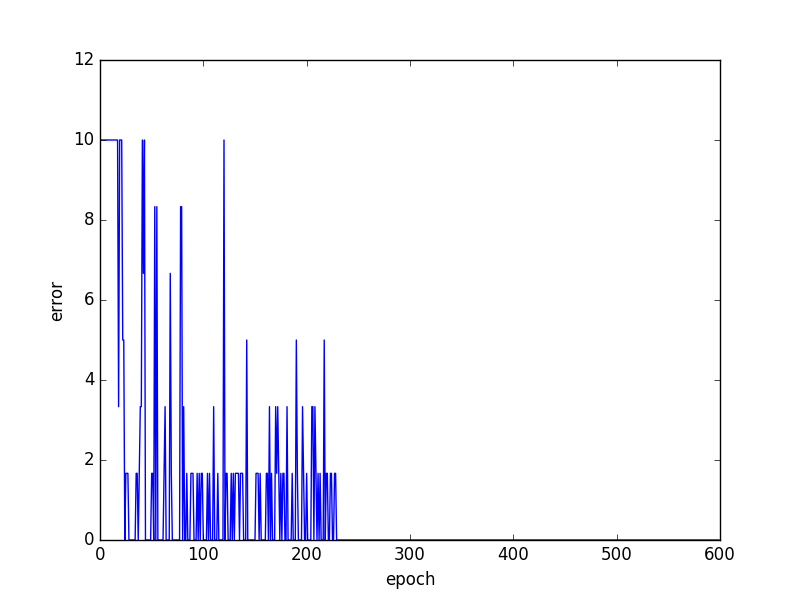
\includegraphics[width=0.47\textwidth]{images/ejecucion2_general/resultados_frav_concatenated/error_nir.png}\label{fig:ejecucion2_frav_clas_train_error_nir}}
\caption{Cost (a) and error (b) at training RGB subset, cost (c) and error (d) at training NIR subset for FRAV (RGB+NIR at classification level) image database.}
\label{fig:ejecucion2_frav_clas_train}
\end{figure}

In RGB and NIR cost training, it got a very low value as in others databases after decreasing its value. Regarding the cost in validation, it gets 0\% in both cases. The difference is that in RGB, this lowest value is gotten twice at epoch 124 and 125 and then the value is increased until it becomes constant at 10\%, what seems to be an overfit. Nevertheless, in the NIR validation error, it oscillates until it gets 0\% value and is constant until the end.\\

The best RGB model is the one obtained at iteration 3347, when 0.0\% is gotten at validation error. The best NIR model is the obtained at iteration 674, the first time that the validation error gets 0\%.

\subsubsection{MFSD database}
The training results obtained with theMFSD database are represented in figure \ref{fig:ejecucion2_mfsd_train}. The cost slowly decreases until it get a desirable cost value, near to 0\%. The validation error curve graph (figure \ref{fig:ejecucion2_mfsd_error}) is not as good as the cost curve. The lower error value is obtained in the first 100 iterations, which is constant and then it increased until 35\%.\\

\begin{figure}[H]
\centering
		\subfigure[Cost at training]{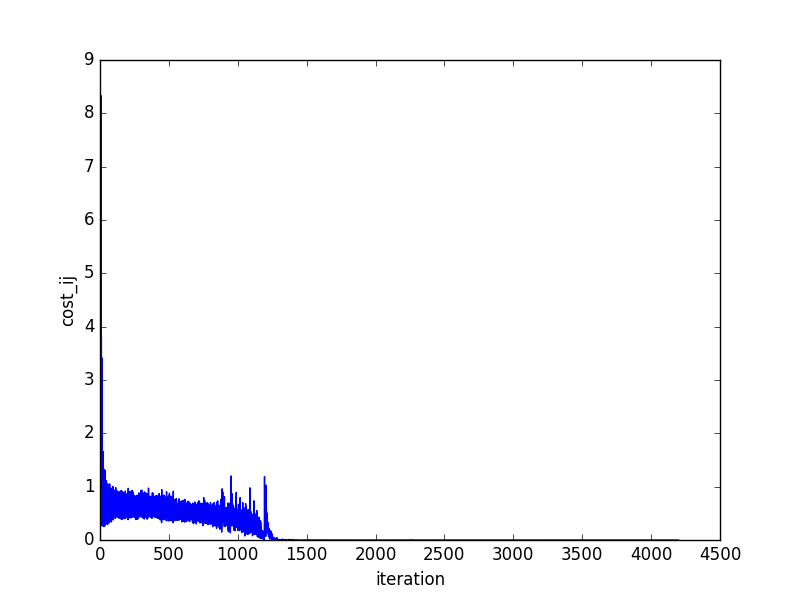
\includegraphics[width=0.47\textwidth]{images/ejecucion2_general/resultados_mfsd/cost.png}\label{fig:ejecucion2_mfsd_cost}}
		\subfigure[Error at validation]{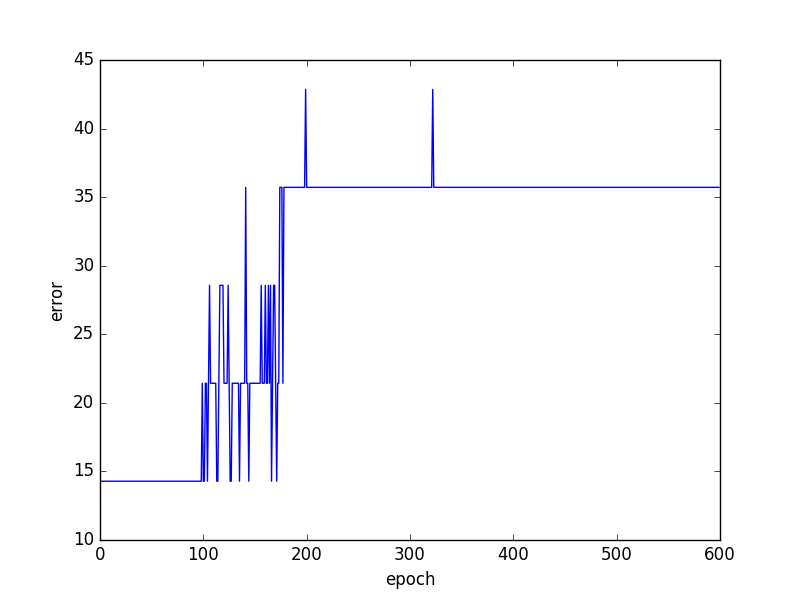
\includegraphics[width=0.47\textwidth]{images/ejecucion2_general/resultados_mfsd/error.png}\label{fig:ejecucion2_mfsd_error}}
\caption{Cost (a) and error (b) at training MFSD image database.}
\label{fig:ejecucion2_mfsd_train}
\end{figure}

The best model is the one obtained at iteration 7 in the first epoch, where the validation error is 14,28\%.

\subsection{Testing process}
From the best CNN model, for each database, A SVM (with linear and RBF kernel), a KNN, a decision tree and a logistic regression have been trained. Furthermore,the testing has been carried out after training a LDA and PCA (which have been trained too for each database) with each classifier.\\

The test performance for each classifier has been executed after chosing the best classifier model.  The results are going to be exposed independently of each database and then compared among all databases.\\

Best obtained results are highlighted in bold in each table.\\

\subsubsection{CASIA Image database}
The results obtained testing the CNN model for CASIA image database are shown. \\

\begin{table}[htb]
\centering
\resizebox{\textwidth}{!}{%
\begin{tabular}{|c|c|c||c|c|c||c|c|c|}
\hline
\rowcolor[HTML]{ECF4FF}
Classifier                                                                   & APCR & BPCR  & \begin{tabular}[|c]{@{}c@{}}Classifier + PCA\\ nº components = 103\end{tabular} & APCR & BPCR  & \begin{tabular}[|c]{@{}c@{}}Classifier + LDA\\ nº components = 1\end{tabular}   & APCR & BPCR  \\ \hline
\begin{tabular}[c]{@{}c@{}}SVM - RBF\\ C = 0.5\end{tabular}                  & 0    & 0.125 & \begin{tabular}[c]{@{}c@{}}SVM - RBF\\ C = 1\end{tabular}                      & 0    & 0.125 & \begin{tabular}[c]{@{}c@{}}SVM - RBF\\ C = 0.5\end{tabular}                    & 0    & 0.125 \\ \hline
\begin{tabular}[c]{@{}c@{}}SVM - lineal\\ C = 0.001\end{tabular}             & 0    & 1     & \begin{tabular}[c]{@{}c@{}}SVM - lineal\\ C = 0.001\end{tabular}               & 0    & 1     & \begin{tabular}[c]{@{}c@{}}SVM - lineal\\ C = 0.005\end{tabular}               & 0    & 1     \\ \hline
\begin{tabular}[c]{@{}c@{}}KNN\\ k = 2\end{tabular}                          & 0    & 0.125 & \begin{tabular}[c]{@{}c@{}}KNN\\ k = 2\end{tabular}                            & 0    & 0.125 & \begin{tabular}[c]{@{}c@{}}KNN\\ k = 4\end{tabular}                            & 0    & 0.125 \\ \hline
\begin{tabular}[c]{@{}c@{}}Decision Tree\\ Depth =  12\end{tabular}          & 0    & 0.5   & \begin{tabular}[c]{@{}c@{}}Decision Tree\\ Depth = 4\end{tabular}              & 0    & 0.125 & \begin{tabular}[c]{@{}c@{}}Decision Tree\\ Depth = 2\end{tabular}              & 0    & 0.125 \\ \hline
\begin{tabular}[c]{@{}c@{}}Logistic Regression\\ l. rate = 0.01\end{tabular} & 0    & 0.125 & \begin{tabular}[c]{@{}c@{}}Logistic Regression\\ l. rate = 0.0001\end{tabular} & 0    & 0.125 & \begin{tabular}[c]{@{}c@{}}Logistic Regression\\ l. rate = 0.0001\end{tabular} & 0    & 0.125 \\ \hline
\end{tabular} }
\caption{APCR and BPCR classifying results using CASIA image database.}
\label{APCR_BPCR_CASIA_im}
\end{table}

In table \ref{APCR_BPCR_CASIA_im} what is  exposed are the APCR and BPCR parameters for each classifier. All the attacks samples are classified correctly because the APCR value is 0. The number of genuine samples misclassified is what changes: it takes value 1 when using SVM with kernel lineal, hence all the positives samples have been misclassified.  And it takes value 0.5 when using the decision tree, whose number of misclassified samples is 5, ( half of the total real samples of the test subset). The rest of the classifiers take a 0.125 APCR value, just one sample is misclassified, the same sample which could be seen in figure \ref{fig:casia_im_miscl}.

Regarding the APCR and the BPCR, it is not possible to get the best combination with which the results are better because most classifiers work correctly.\\

\begin{figure}[htb]
\centering
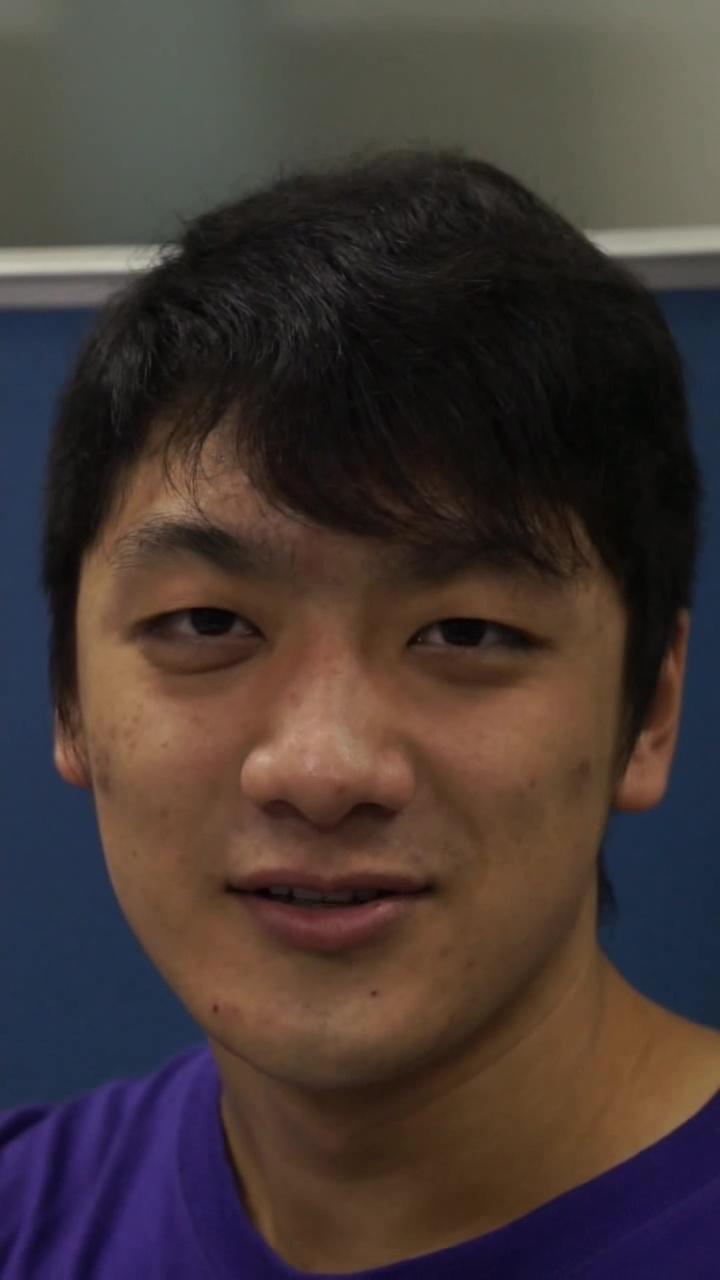
\includegraphics[width=0.2\textwidth]{images_databases/casia_real_41.jpg}
\caption{Casia image misclassified sample.} \label{fig:casia_im_miscl}
\end{figure}

Figure \ref{fig:CASIA_im_FAR_FRR} represents  FAR and FRR curves, from which is obtained a 0,025 EER at 0,015 threshold. The EER obtained is a desirable result, on the contrary, the threshold is low, it is not usually used a 0,015 threshold.

\begin{figure}[htb]
\centering
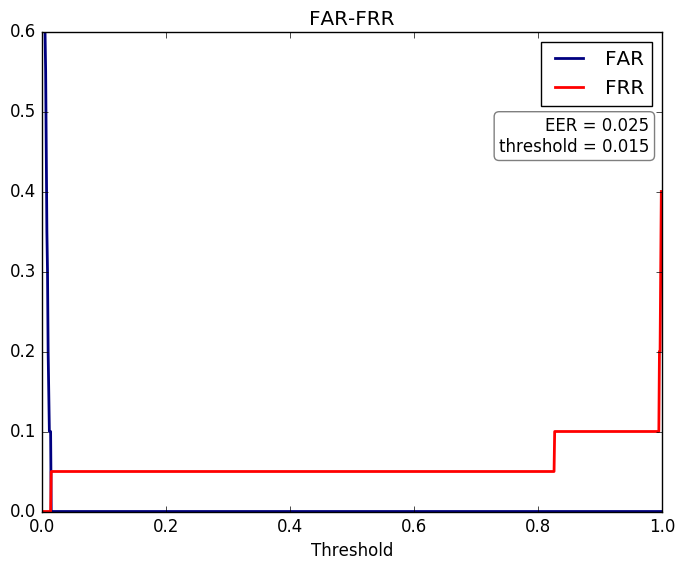
\includegraphics[width=0.5\textwidth]{images/FAR-FRR/CASIA_im_SVM_RBF_FAR_FRR.png}
\caption{FAR-FRR curve of CASIA image database using SVM (RBF kernel).} \label{fig:CASIA_im_FAR_FRR}
\end{figure}


\subsubsection{CASIA Video database}
Next analysed results are from the CASIA video database.\\

\begin{table}[htb]
\centering
\resizebox{\textwidth}{!}{%
\begin{tabular}{|c|c|c||c|c|c||c|c|c|}
\hline
\rowcolor[HTML]{ECF4FF}
Classifier                                                                   & APCR & BPCR & \begin{tabular}[|c]{@{}c@{}}Classifier + PCA\\ nº components = 283\end{tabular} & APCR & BPCR & \begin{tabular}[|c]{@{}c@{}}Classifier + LDA\\ nº components = 1\end{tabular}  & APCR & BPCR \\ \hline
\begin{tabular}[c]{@{}c@{}}SVM - RBF\\ C = 0.1\end{tabular}                  & 0.14 & 0.53 & \begin{tabular}[c]{@{}c@{}}SVM - RBF\\ C = 0.5\end{tabular}                    & 0.17 & 0.46 & \begin{tabular}[c]{@{}c@{}}SVM - RBF\\ C = 0.05\end{tabular}                  & \textbf{0.16} & \textbf{0.44} \\ \hline
\begin{tabular}[c]{@{}c@{}}SVM - lineal\\ C = 0.001\end{tabular}             & 0    & 1    & \begin{tabular}[c]{@{}c@{}}SVM - lineal\\ C = 0.001\end{tabular}               & 0    & 1    & \begin{tabular}[c]{@{}c@{}}SVM - lineal\\ C = 0.001\end{tabular}              & 0    & 1    \\ \hline
\begin{tabular}[c]{@{}c@{}}KNN\\ k = 2\end{tabular}                          & 0.19 & 0.42 & \begin{tabular}[c]{@{}c@{}}KNN\\ k = 2\end{tabular}                            & 0.2  & 0.42 & \begin{tabular}[c]{@{}c@{}}KNN\\ k = 2\end{tabular}                           & 0.16 & 0.47 \\ \hline
\begin{tabular}[c]{@{}c@{}}Decision Tree\\ Depth =  2\end{tabular}           & 0.19 & 0.49 & \begin{tabular}[c]{@{}c@{}}Decision Tree\\ Depth = 2\end{tabular}              & 0.15 & 0.53 & \begin{tabular}[c]{@{}c@{}}Decision Tree\\ Depth = 2\end{tabular}             & 0.15 & 0.46 \\ \hline
\begin{tabular}[c]{@{}c@{}}Logistic Regression\\ l. rate = 0.01\end{tabular} & 0.15 & 0.49 & \begin{tabular}[c]{@{}c@{}}Logistic Regression\\ l. rate = 0.005\end{tabular}  & 0.23 & 0.34 & \begin{tabular}[c]{@{}c@{}}Logistic Regression\\ l. rate = 0.005\end{tabular} & 0.23 & 0.37 \\ \hline
\end{tabular} }
\caption{APCR and BPCR classifying results using CASIA video database.}
\label{APCR_BPCR_CASIA_vid}
\end{table}

In table \ref{APCR_BPCR_CASIA_vid} APCR and BPCR results are summarized. The best result has been obtained with SVM classifier and kernel RBF (C= 0.05) after applying LDA with 1 component. The worst values obtained are the SVM with lineal kernel, even if PCA or LDA have been used, because all the positives samples have been classified as negative. \\

From the table it is not possible to know if LDA and PCA are significant because with some classifiers APCR and BPCR results have been improved or worsened.\\

Also The last conclusion that could be obtained from the table is that the attack samples are better classified than the genuine samples.This is due to the fact that it has been trained with more negative samples.\\

Figure \ref{fig:CASIA_vid_FAR_FRR} represents the FAR-FRR curve of the best obtained model: CNN architecture and using LDA with SVM RBF kernel. From the figure, the Equal Error Rate obtained value is 0.115, it is a improvable value; EER is obtained at 0,64 threshold.


\begin{figure}[htb]
\centering
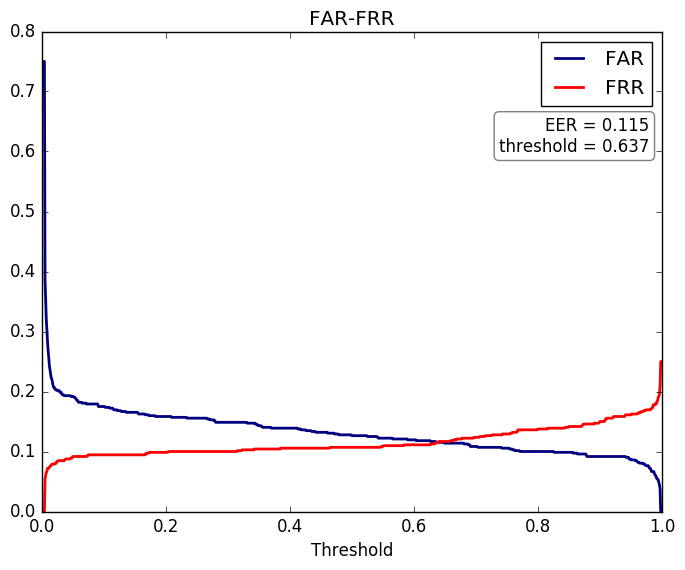
\includegraphics[width=0.5\textwidth]{images/FAR-FRR/Casia_vid_LDA_SVM_RBF_FAR_FRR.png}
\caption{FAR-FRR curve of CASIA videos database using LDA and SVM (RBF kernel).} \label{fig:CASIA_vid_FAR_FRR}
\end{figure}

\subsubsection{RGB FRAV database}
The RGB FRAV database results are presented and analyzed.\\

\begin{table}[htb]
\centering
\resizebox{\textwidth}{!}{%
\begin{tabular}{|c|c|c||c|c|c||c|c|c|}
\hline
\rowcolor[HTML]{ECF4FF}
Classifier                                                                   & APCR & BPCR & \begin{tabular}[|c]{@{}c@{}}Classifier + PCA\\ nº components = 463\end{tabular} & APCR & BPCR & \begin{tabular}[|c]{@{}c@{}}Classifier + LDA\\ nº components = 1\end{tabular}  & APCR & BPCR \\ \hline
\begin{tabular}[c]{@{}c@{}}SVM - RBF\\ C = 0.5\end{tabular}                  & 0.06 & 0.06 & \begin{tabular}[c]{@{}c@{}}SVM - RBF\\ C = 1\end{tabular}                      & \textbf{0.04} & \textbf{0.06} & \begin{tabular}[c]{@{}c@{}}SVM - RBF\\ C = 0.1\end{tabular}                   & 0.05 & 0.06 \\ \hline
\begin{tabular}[c]{@{}c@{}}SVM - lineal\\ C = 0.005\end{tabular}             & 0    & 1    & \begin{tabular}[c]{@{}c@{}}SVM - lineal\\ C = 0.005\end{tabular}               & 0    & 1    & \begin{tabular}[c]{@{}c@{}}SVM - lineal\\ C = 0.5\end{tabular}                & 0.05 & 0.06 \\ \hline
\begin{tabular}[c]{@{}c@{}}KNN\\ k = 16\end{tabular}                         & 0.07 & 0.06 & \begin{tabular}[c]{@{}c@{}}KNN\\ k = 26\end{tabular}                           & 0.06 & 0.06 & \begin{tabular}[c]{@{}c@{}}KNN\\ k = 20\end{tabular}                          & 0.05 & 0.06 \\ \hline
\begin{tabular}[c]{@{}c@{}}Decision Tree\\ Depth =  2\end{tabular}           & 0.04 & 0.11 & \begin{tabular}[c]{@{}c@{}}Decision Tree\\ Depth = 2\end{tabular}              & 0.06 & 0.11 & \begin{tabular}[c]{@{}c@{}}Decision Tree\\ Depth = 2\end{tabular}             & 0.06 & 0.06 \\ \hline
\begin{tabular}[c]{@{}c@{}}Logistic Regression\\ l. rate = 0.01\end{tabular} & 0.01 & 0.17 & \begin{tabular}[c]{@{}c@{}}Logistic Regression\\ l. rate = 0.05\end{tabular}   & 0.06 & 0.06 & \begin{tabular}[c]{@{}c@{}}Logistic Regression\\ l. rate = 0.005\end{tabular} & 0.06 & 0.06 \\ \hline
\end{tabular} }
\caption{APCR and BPCR classifying results using FRAV RGB database.}
\label{APCR_BPCR_FRAV}
\end{table}

APCR and BPCR results are in table \ref{APCR_BPCR_FRAV}. In general, results are very good because values are lower than 0.5. With SVM lineal kernel, all the samples are classified as negatives except when it has been used when LDA, those results are as good as the ones obtained with RBF kernel.\\

The best  result is obtained when SVM with RBF kernel has been used with C = 1 and using LDA with 1 component. LDA improves the results obtained when neither PCA nor just the classifier have been used, although the improvement is not much.\\

The misclassified samples are repeated among the classifiers. The two samples shown in figure \ref{fig:frav_miscl} represent the two most misclassified images, almost every classifier has classified it incorrectly.\\

\begin{figure}[htb]
\centering
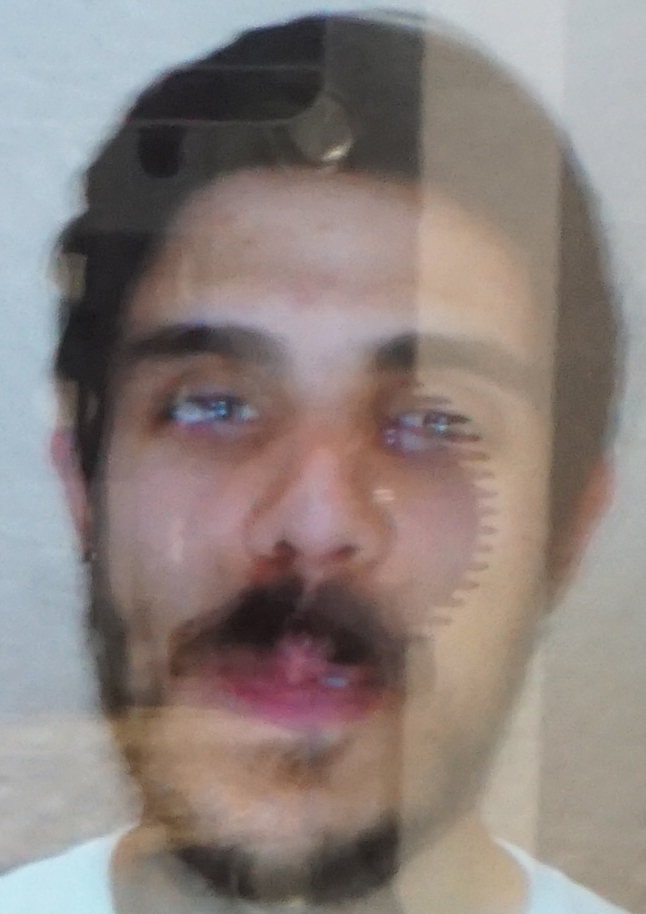
\includegraphics[width=0.2\textwidth]{images_databases/frav_tablet_109.JPG}
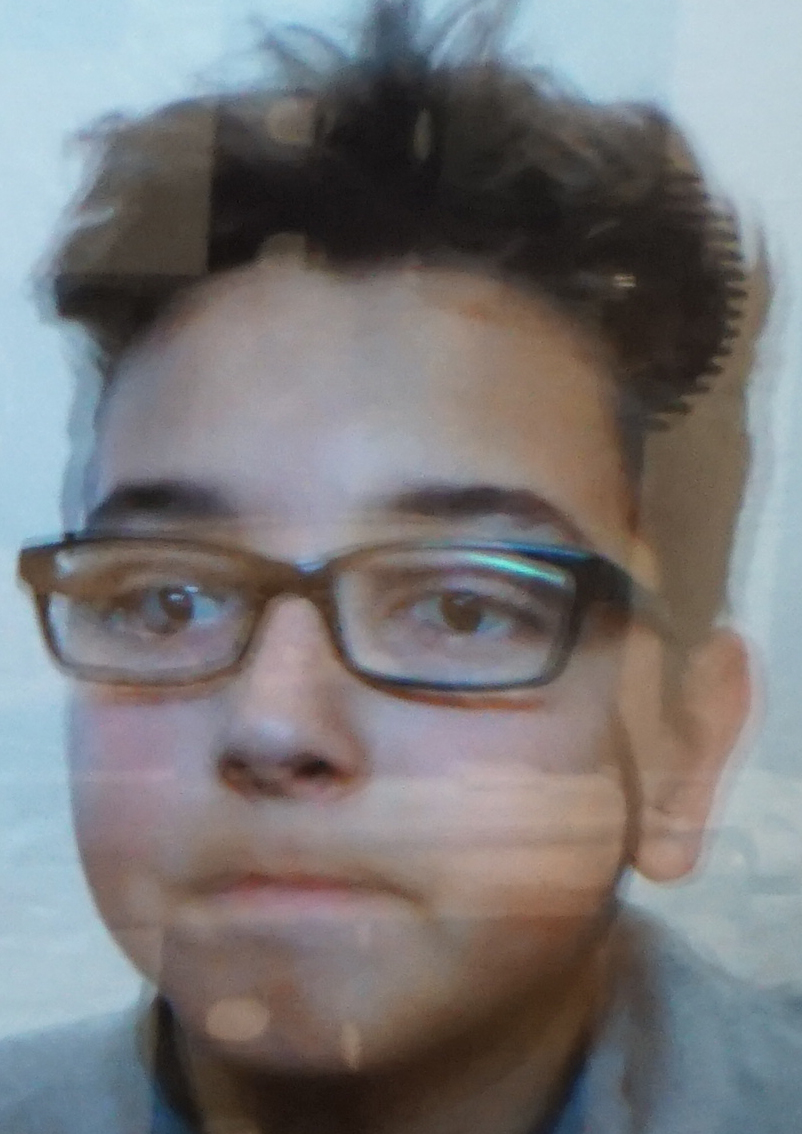
\includegraphics[width=0.2\textwidth]{images_databases/frav_tablet_162.JPG}
%('False Positive: ', 'databases/from/attack_04/tablet_162.JPG') ('False Positive: ', 'databases/from/attack_04/tablet_109.JPG')
\caption{RGB FRAV misclassified samples.} \label{fig:frav_miscl}
\end{figure}

The FAR-FRR graph is represented in figure \ref{fig:RGB_FRAV_FAR_FRR} from which the EER value acquired is 0.022, a satisfactory value, at 0.954 threshold. The performance of the FAR and FRR curves is acceptable because the values obtained are low, and that means that the false positives and false negatives are a small quantity.

\begin{figure}[htb]
\centering
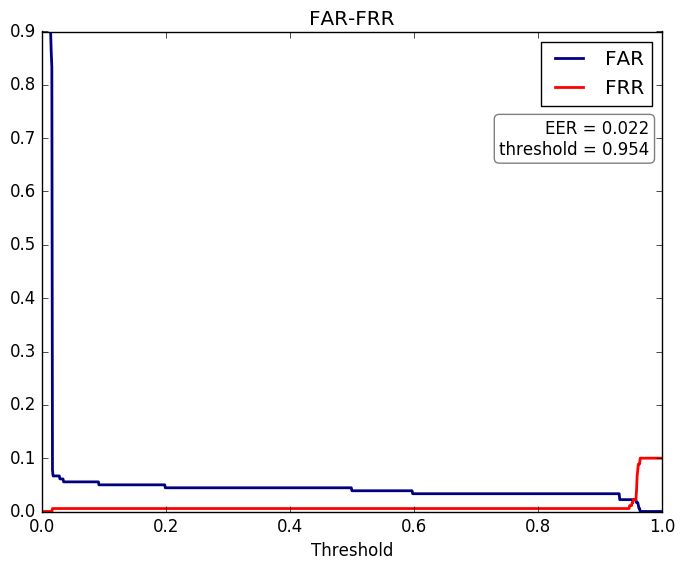
\includegraphics[width=0.5\textwidth]{images/FAR-FRR/FRAV_LDA_SVM_RBF_FAR_FRR.png}
\caption{FAR-FRR curve of RGB FRAV database using LDA and SVM (RBF kernel).} \label{fig:RGB_FRAV_FAR_FRR}
\end{figure}


\subsubsection{FRAV RGB+NIR (feature level) database}
Results obtained at classifying RGB+NIR (feature level) database are shown next.\\

\begin{table}[htb]
\centering
\resizebox{\textwidth}{!}{%
\begin{tabular}{|c|c|c||c|c|c||c|c|c|}
\hline
\rowcolor[HTML]{ECF4FF}
Classifier                                                                   & APCR & BPCR & \begin{tabular}[|c]{@{}c@{}}Classifier + PCA\\ nº components = 463\end{tabular} & APCR & BPCR & \begin{tabular}[|c]{@{}c@{}}Classifier + LDA\\ nº components = 1\end{tabular} & APCR & BPCR \\ \hline
\begin{tabular}[c]{@{}c@{}}SVM - RBF\\ C = 2\end{tabular}                    & 0.02 & 0    & \begin{tabular}[c]{@{}c@{}}SVM - RBF\\ C = 5\end{tabular}                      & 0.02 & 0    & \begin{tabular}[c]{@{}c@{}}SVM - RBF\\ C = 0.1\end{tabular}                  & 0.04 & 0    \\ \hline
\begin{tabular}[c]{@{}c@{}}SVM - lineal\\ C = 0.005\end{tabular}             & 0    & 1    & \begin{tabular}[c]{@{}c@{}}SVM - lineal\\ C = 0.001\end{tabular}               & 0    & 1    & \begin{tabular}[c]{@{}c@{}}SVM - lineal\\ C = 10\end{tabular}                & 0.05 & 0    \\ \hline
\begin{tabular}[c]{@{}c@{}}KNN\\ k = 6\end{tabular}                          & 0.09 & 0    & \begin{tabular}[c]{@{}c@{}}KNN\\ k = 12\end{tabular}                           & 0.12 & 0    & \begin{tabular}[c]{@{}c@{}}KNN\\ k = 10\end{tabular}                         & 0.04 & 0    \\ \hline
\begin{tabular}[c]{@{}c@{}}Decision Tree\\ Depth =  2\end{tabular}           & \textbf{0}    & \textbf{0}    & \begin{tabular}[c]{@{}c@{}}Decision Tree\\ Depth = 2\end{tabular}              & 0.01 & 0    & \begin{tabular}[c]{@{}c@{}}Decision Tree\\ Depth = 2\end{tabular}            & 0.05 & 0    \\ \hline
\begin{tabular}[c]{@{}c@{}}Logistic Regression\\ l. rate = 0.01\end{tabular} & \textbf{0}    & \textbf{0}    & \begin{tabular}[c]{@{}c@{}}Logistic Regression\\ l. rate = 0.05\end{tabular}   & 0.06 & 0    & \begin{tabular}[c]{@{}c@{}}Logistic Regression\\ l. rate = 0.05\end{tabular} & 0.07 & 0    \\ \hline
\end{tabular} }
\caption{APCR and BPCR classifying results using FRAV RGB+NIR (feature level) database.}
\label{APCR_BPCR_FRAV_feature}
\end{table}

Table \ref{APCR_BPCR_FRAV_feature} shows the APCR and BPCR values that have been obtained for each classifier. Except for SVM with lineal kernel, which has classified all the samples as negatives when just the classifier has been used or if PCA has been applied, classifications have obtained good results. The APCR and BPCR values are very low, close to 0. In fact, the Decision Tree and logistic regression classify correctly all the samples because APCR and BPCR are equal to 0. \\

PCA and LDA have barely improved results. SVM lineal with LDA does not classify all the samples as negatives. When PCA and LDA is applied with logistic regression and Decision tree, the classification is not perfect as it is when none is applied.\\

In general, the same samples are misclassified in the classification tasks. The two most misclassified samples are represented in figure \ref{fig:frav_feat_miscl}.\\

\begin{figure}[htb]
\centering
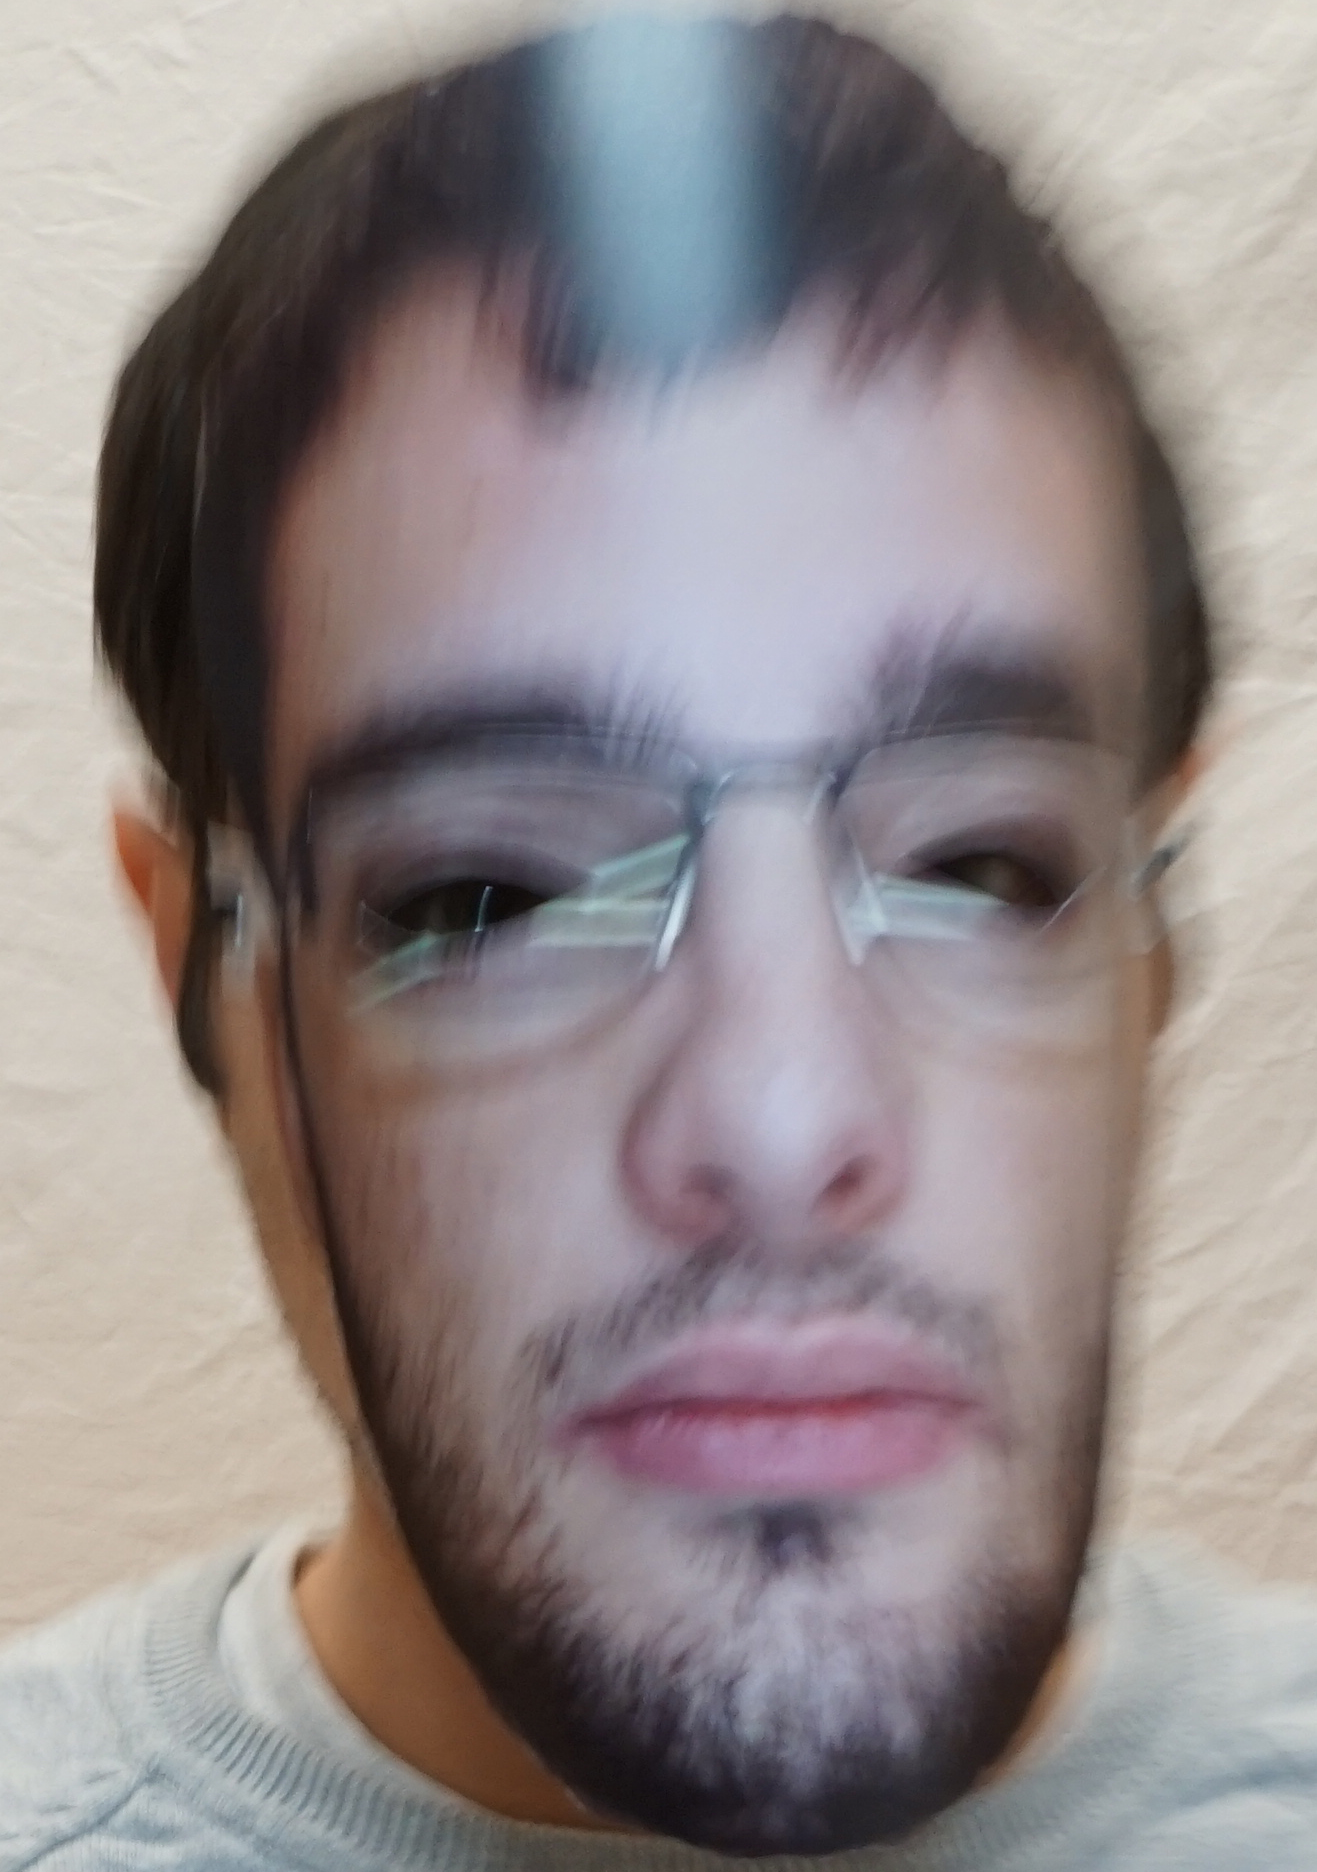
\includegraphics[width=0.2\textwidth]{images_databases/frav_rgb_151.JPG}
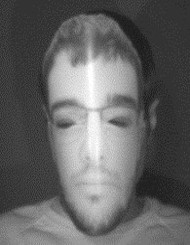
\includegraphics[width=0.2\textwidth]{images_databases/frav_nir_151.jpg}
\\
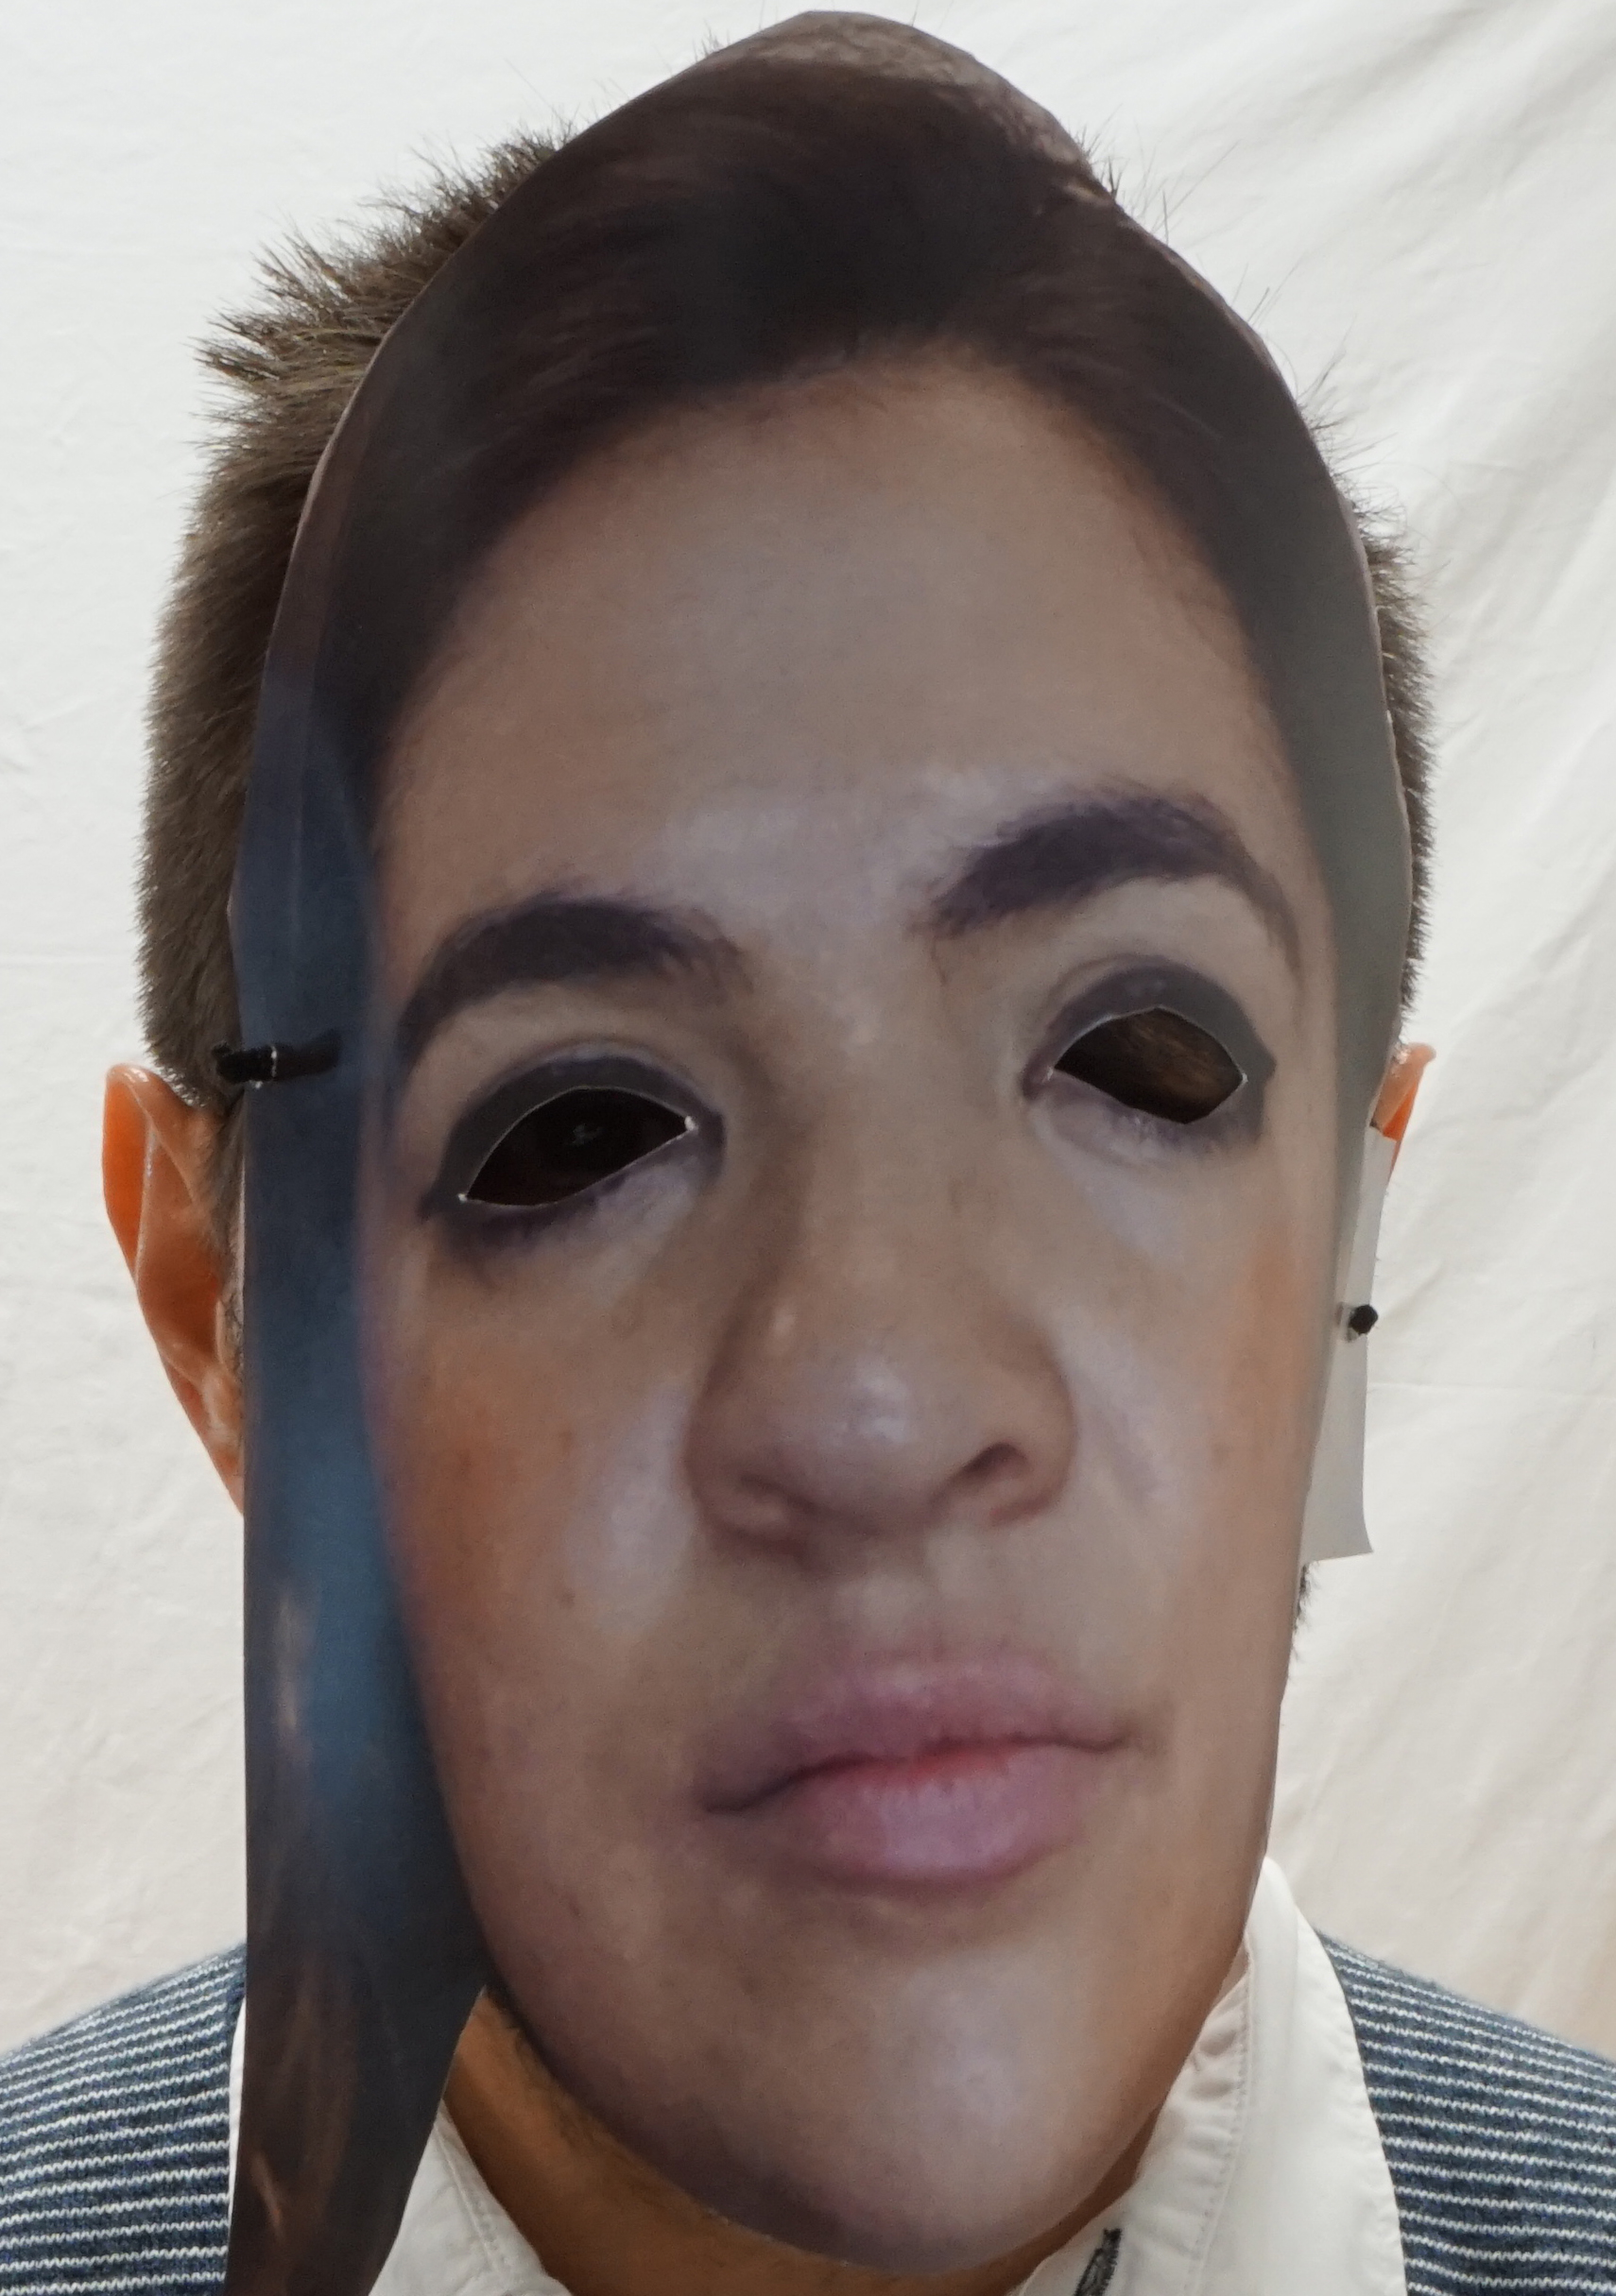
\includegraphics[width=0.2\textwidth]{images_databases/frav_rgb_128.JPG}
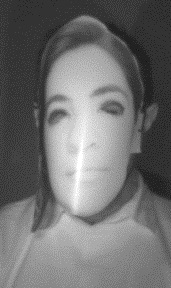
\includegraphics[width=0.2\textwidth]{images_databases/frav_nir_128.jpg}
%('False Positive: ', 'databases/RGB_NIR/RGB/attack_03/151.JPG') ('False Positive: ', 'databases/RGB_NIR/RGB/attack_03/128.JPG')
\caption{RGB+NIR FRAV (feature level) misclassified samples.} \label{fig:frav_feat_miscl}
\end{figure}

The perfect performance could be also demonstrated in figure \ref{figures:FAR-FRR-FRAV_FEAT}, where FAR and FRR curves are plot when logistic regression and Decision Tree classifiers are used. In both cases, because of the perfect classification, the EER value obtained is 0.

\begin{figure}[htb]
    \centering
	\subfigure[logistic regression classifier]{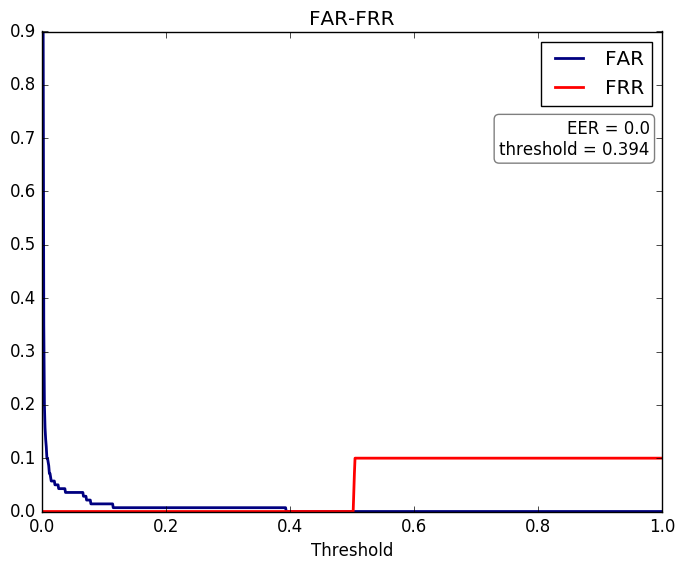
\includegraphics[width=0.47\textwidth]{images/FAR-FRR/FRAV_feat_SOFTMAX_FAR_FRR.png} }
	\subfigure[Decision Tree classifier]{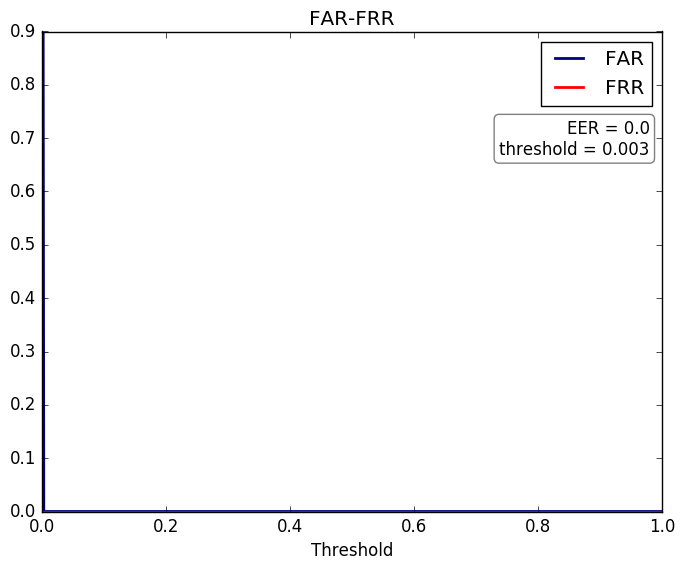
\includegraphics[width=0.47\textwidth]{images/FAR-FRR/FRAV_feat_DecisionTree_FAR_FRR.png} }

    \caption{FAR-FRR curve for RGB+NIR FRAV database (feature level).} \label{figures:FAR-FRR-FRAV_FEAT}
\end{figure}

\subsubsection{FRAV RGB+NIR (classification level) database}
Results obtained when the RGB+NIR FRAV database (classification level) is used are described below.\\
\begin{table}[htb]
\centering
\resizebox{\textwidth}{!}{%
\begin{tabular}{|c|c|c||c|c|c||c|c|c|}
\hline
\rowcolor[HTML]{ECF4FF}
Classifier                                                                   & APCR & BPCR & \begin{tabular}[|c]{@{}c@{}}Classifier + PCA\\ nº components = 463\end{tabular} & APCR & BPCR & \begin{tabular}[|c]{@{}c@{}}Classifier + LDA\\ nº components = 1\end{tabular}  & APCR & BPCR \\ \hline
\begin{tabular}[c]{@{}c@{}}SVM - RBF\\ C = 10\end{tabular}                   & 0.01 & 0    & \begin{tabular}[c]{@{}c@{}}SVM - RBF\\ C = 1\end{tabular}                      & 0.02 & 0    & \begin{tabular}[c]{@{}c@{}}SVM - RBF\\ C = 2\end{tabular}                     & 0.01 & 0    \\ \hline
\begin{tabular}[c]{@{}c@{}}SVM - lineal\\ C = 0.001\end{tabular}             & 0    & 1    & \begin{tabular}[c]{@{}c@{}}SVM - lineal\\ C = 0.001\end{tabular}               & 0    & 1    & \begin{tabular}[c]{@{}c@{}}SVM - lineal\\ C = 1\end{tabular}                  & 0.01 & 0    \\ \hline
\begin{tabular}[c]{@{}c@{}}KNN\\ k = 6\end{tabular}                          & 0.32 & 0    & \begin{tabular}[c]{@{}c@{}}KNN\\ k = 14\end{tabular}                           & 0.04 & 0    & \begin{tabular}[c]{@{}c@{}}KNN\\ k = 6\end{tabular}                           & 0.01 & 0    \\ \hline
\begin{tabular}[c]{@{}c@{}}Decision Tree\\ Depth =  2\end{tabular}           & 0.04 & 0.07 & \begin{tabular}[c]{@{}c@{}}Decision Tree\\ Depth = 2\end{tabular}              & 0.05 & 0.07 & \begin{tabular}[c]{@{}c@{}}Decision Tree\\ Depth = 2\end{tabular}             & 0.01 & 0    \\ \hline
\begin{tabular}[c]{@{}c@{}}Logistic Regression\\ l. rate = 0.01\end{tabular} & 0    & 0.29 & \begin{tabular}[c]{@{}c@{}}Logistic Regression\\ l. rate = 0.05\end{tabular}   & 0.07 & 0    & \begin{tabular}[c]{@{}c@{}}Logistic Regression\\ l. rate = 0.005\end{tabular} & 0.02 & 0    \\ \hline
\end{tabular} }
\caption{APCR and BPCR classifying results using FRAV RGB+NIR (classification level) database.}
\label{APCR_BPCR_FRAV_class}
\end{table}

APCER and BPCER results are summarized in table \ref{APCR_BPCR_FRAV_class}. Results are closer to 0, but no classifier classifies perfectly. When using LDA, one can see that APCR results improve and the BPCR results are perfect.\\

SVM lineal classifier classifies incorrectly positives samples although PCA is used too. With LDA, that does not happen.\\

In most cases, classifiers just mis-classify one sample, the same sample represented in figure \ref{fig:frav_clas_miscl}. Classifiers that mis-classify more than one sample, the sample \ref{fig:frav_clas_miscl} is one of the misclassified.\\

\begin{figure}[htb]
\centering
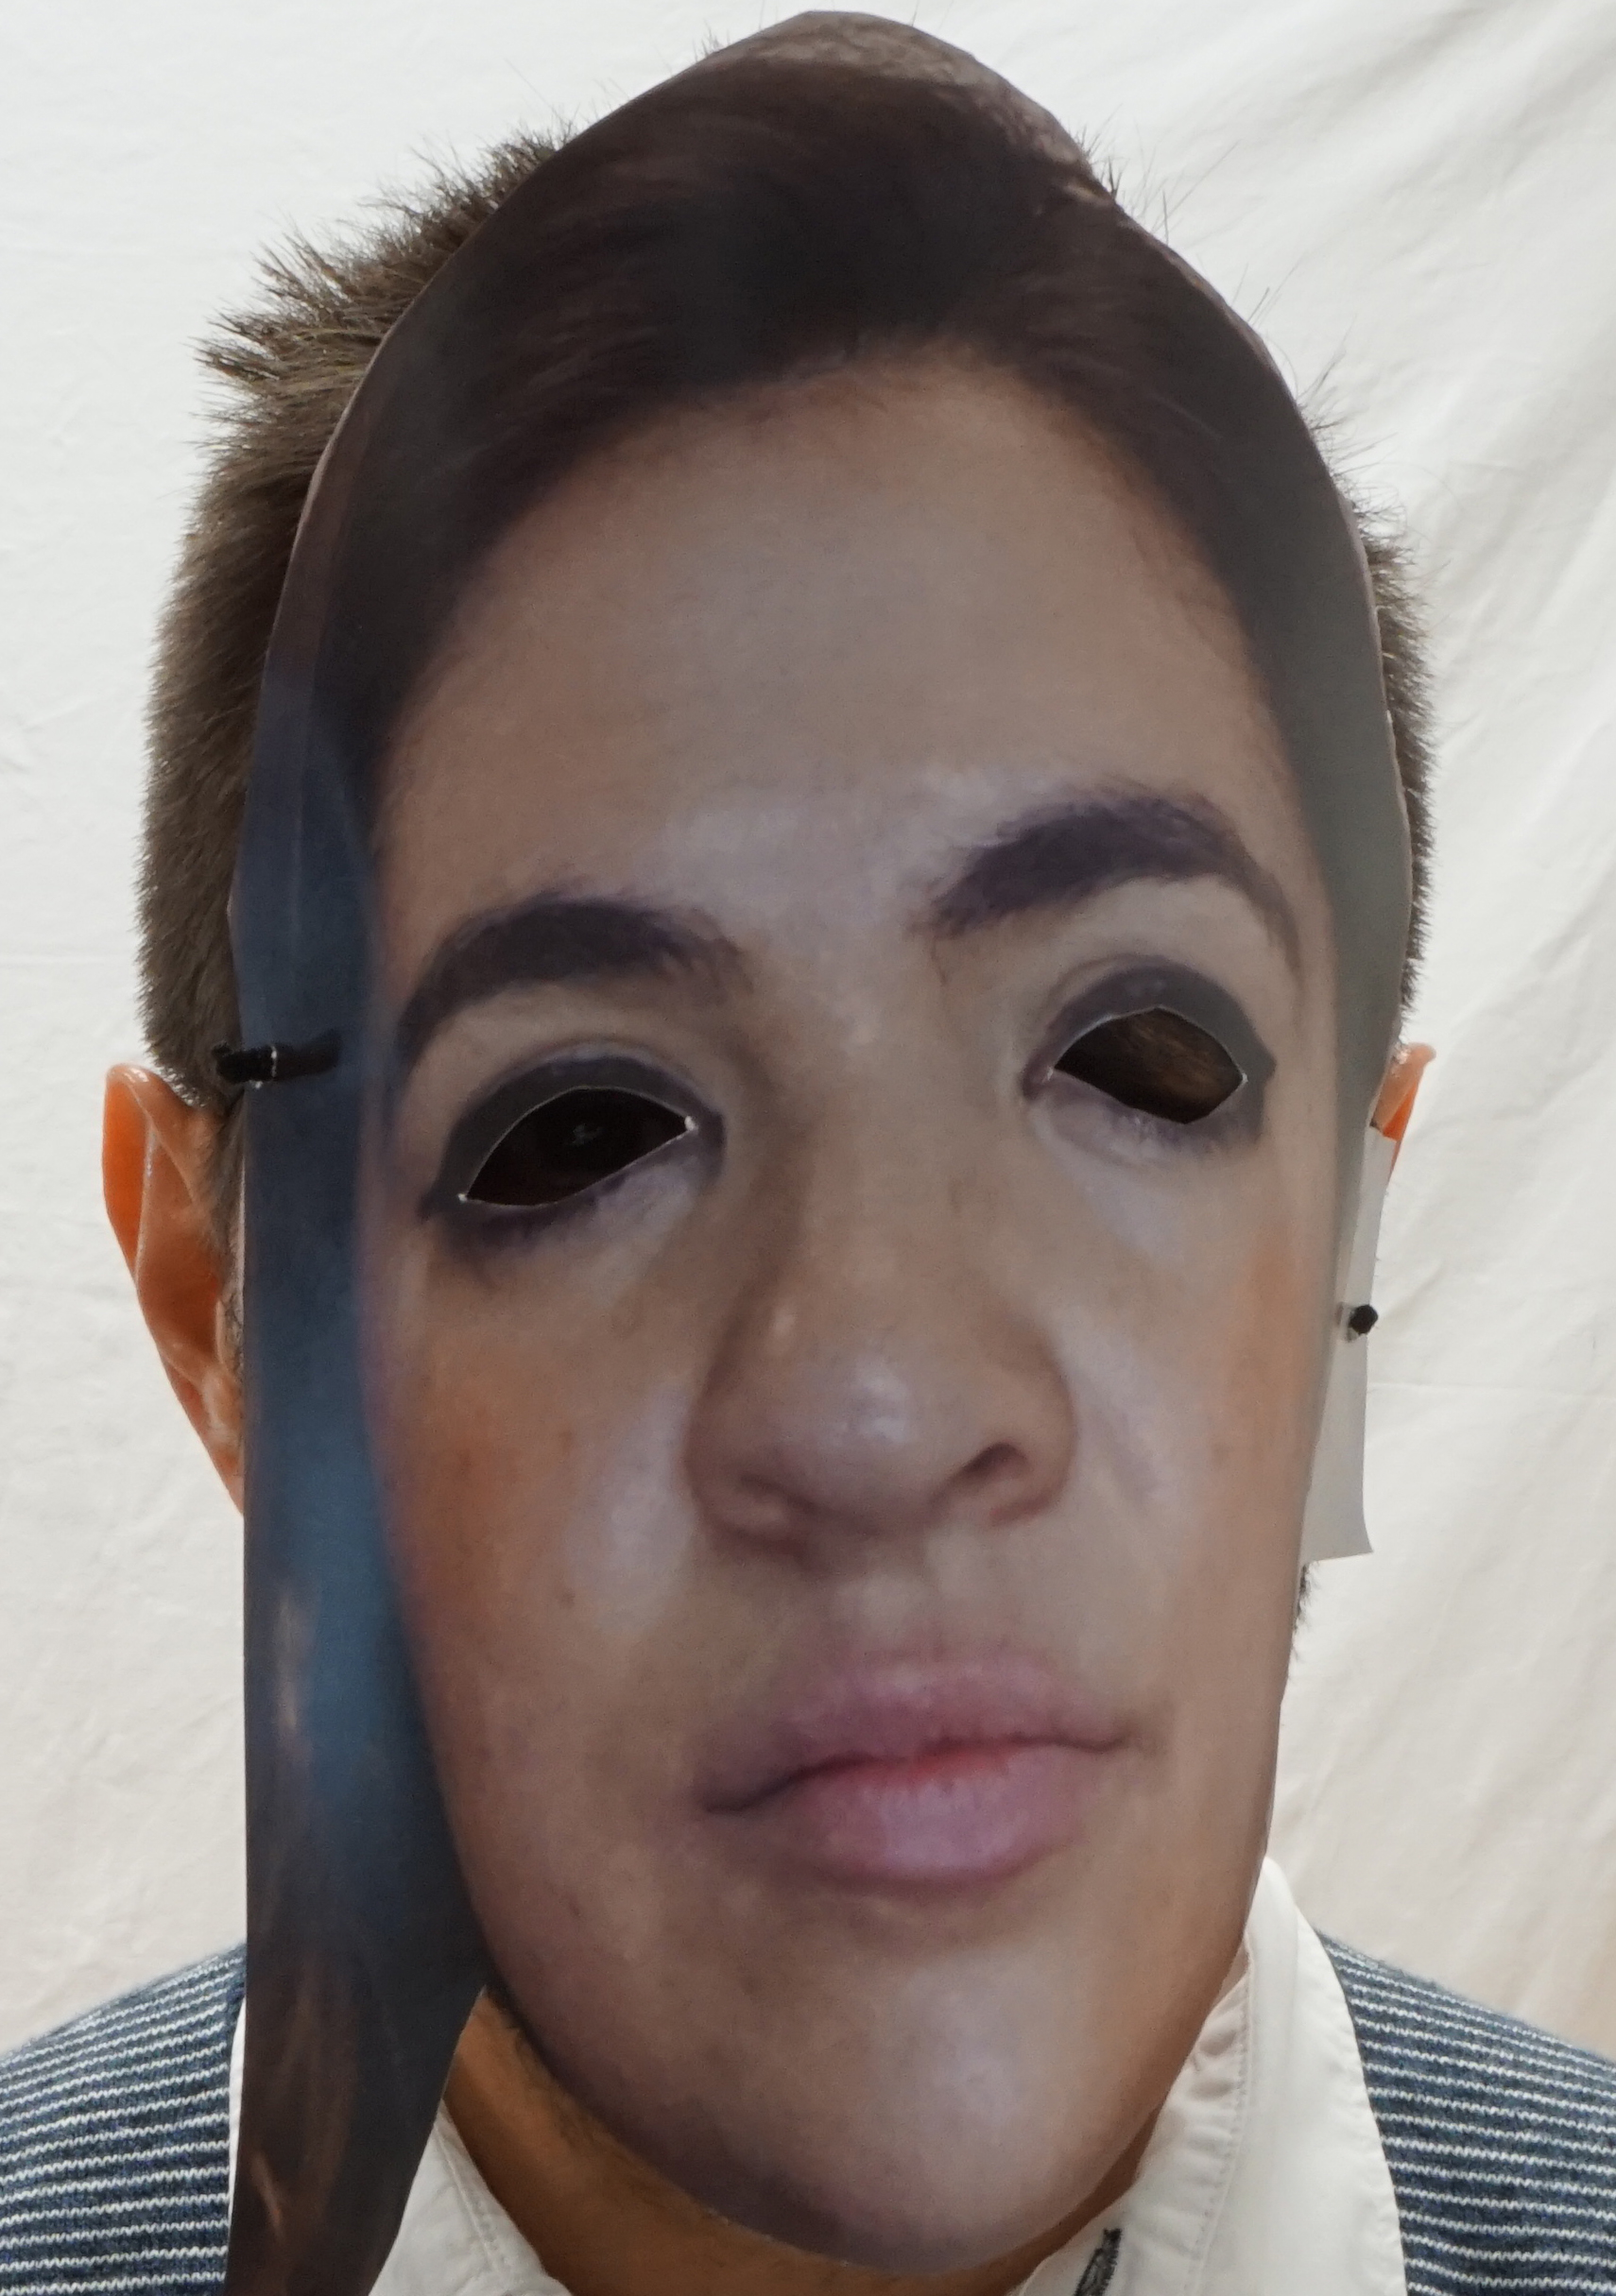
\includegraphics[width=0.2\textwidth]{images_databases/frav_rgb_128.JPG}
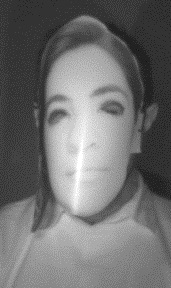
\includegraphics[width=0.2\textwidth]{images_databases/frav_nir_128.jpg}
%('False Positive: ', 'databases/RGB_NIR/RGB/attack_03/128.JPG')
\caption{RGB+NIR FRAV (classification level) misclassified samples.} \label{fig:frav_clas_miscl}
\end{figure}

There are various classifiers which realize the best performance, FAR-FRR curve it is illustrated for SVM (RBF kernel) with LDA method in figure \ref{fig:RGB_FRAV_clas_FAR_FRR}. The result obtained is acceptable, a 0,004 ERR. The number of incorrectly classified samples is low.

\begin{figure}[htb]
\centering
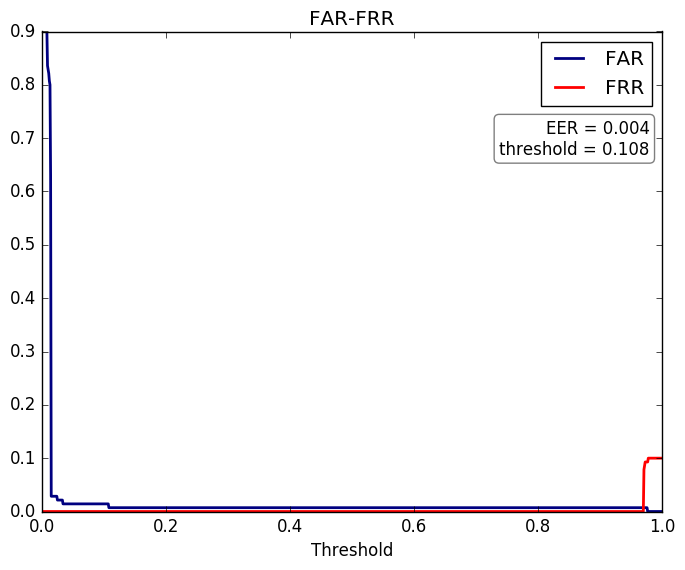
\includegraphics[width=0.5\textwidth]{images/FAR-FRR/FRAV_clas_LDA_SVM_RBF_FAR_FRR.png}
\caption{FAR-FRR curve of RGB+NIR FRAV (classification level) database using LDA and SVM (RBF kernel).} \label{fig:RGB_FRAV_clas_FAR_FRR}
\end{figure}

\subsubsection{MFSD-MSU database}
MFSD-MSU database results are described following.\\

\begin{table}[htb]
\centering
\resizebox{\textwidth}{!}{%
\begin{tabular}{|c|c|c||c|c|c||c|c|c|}
\hline
\rowcolor[HTML]{ECF4FF}
Classifier                                                                   & APCR & BPCR & \begin{tabular}[|c]{@{}c@{}}Classifier + PCA\\ nº components = 463\end{tabular} & APCR & BPCR & \begin{tabular}[|c]{@{}c@{}}Classifier + LDA\\ nº components = 1\end{tabular}   & APCR & BPCR \\ \hline
\begin{tabular}[c]{@{}c@{}}SVM - RBF\\ C = 0.01\end{tabular}                 & 0    & 1    & \begin{tabular}[c]{@{}c@{}}SVM - RBF\\ C = 0.001\end{tabular}                  & 0    & 1    & \begin{tabular}[c]{@{}c@{}}SVM - RBF\\ C = 1\end{tabular}                      & 0    & 1    \\ \hline
\begin{tabular}[c]{@{}c@{}}SVM - lineal\\ C = 0.001\end{tabular}             & 0    & 1    & \begin{tabular}[c]{@{}c@{}}SVM - lineal\\ C = 0.001\end{tabular}               & 0    & 1    & \begin{tabular}[c]{@{}c@{}}SVM - lineal\\ C = 10\end{tabular}                  & 0    & 1    \\ \hline
\begin{tabular}[c]{@{}c@{}}KNN\\ k = 24\end{tabular}                         & 0    & 1    & \begin{tabular}[c]{@{}c@{}}KNN\\ k = 30\end{tabular}                           & 0    & 1    & \begin{tabular}[c]{@{}c@{}}KNN\\ k = 30\end{tabular}                           & 0    & 1    \\ \hline
\begin{tabular}[c]{@{}c@{}}Decision Tree\\ Depth =  12\end{tabular}          & 0    & 1    & \begin{tabular}[c]{@{}c@{}}Decision Tree\\ Depth = 2\end{tabular}              & 0    & 1    & \begin{tabular}[c]{@{}c@{}}Decision Tree\\ Depth = 2\end{tabular}              & 0    & 1    \\ \hline
\begin{tabular}[c]{@{}c@{}}Logistic Regression\\ l. rate = 0.01\end{tabular} & 0    & 1    & \begin{tabular}[c]{@{}c@{}}Logistic Regression\\ l. rate = 0.0001\end{tabular} & 0    & 1    & \begin{tabular}[c]{@{}c@{}}Logistic Regression\\ l. rate = 0.0001\end{tabular} & 0    & 1    \\ \hline
\end{tabular} }
\caption{APCR and BPCR classifying results using MFSD-MSU database.}
\label{APCR_BPCR_MFSD}
\end{table}

The classification with this database is not accurate because all the samples are classified as negatives, as could be seen in table \ref{APCR_BPCR_MFSD} where , independently of the classifier or if LDA and PCA are used, the BPCR value is always 1 and the APCR value is 0.\\

Because of the similarity in results, only FAR-FRR curve of SVM with RBF is demonstrated. Figure \ref{fig:MFSD_FAR_FRR} showa FAR-FRR curve. The result obtained is an 0,089 EER, it is not an unacceptable value, but it is due to the fact that all samples are classified as negative samples.

\begin{figure}[htb]
\centering
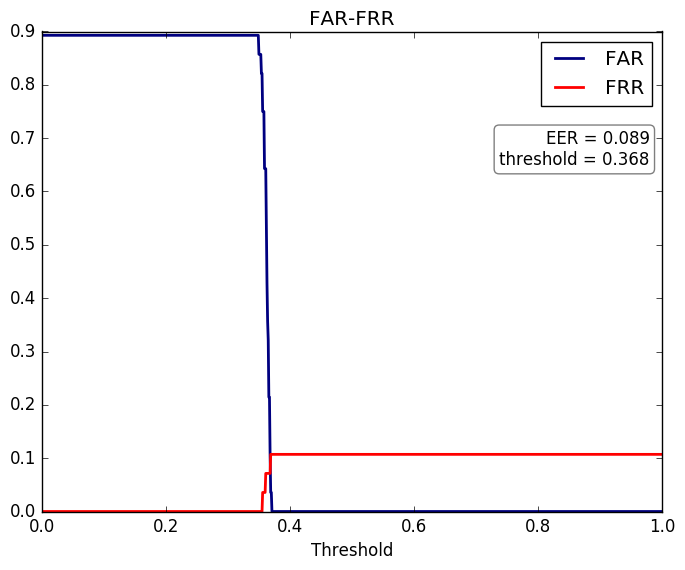
\includegraphics[width=0.5\textwidth]{images/FAR-FRR/MFSD_SVM_RBF_FAR_FRR.png}
\caption{FAR-FRR curve of MFSD database using SVM with RBF kernel.} \label{fig:MFSD_FAR_FRR}
\end{figure}



\subsection{Comparative among databases}
In this section it is going to discuss databases classification in common.

\subsubsection{CASIAs databases}
A comparative between the obtained results of the two CASIAs databases: Image and Videos. In order to do so, KNN classifier is going to be used to compare them.\\

\begin{figure}[htb]
\centering
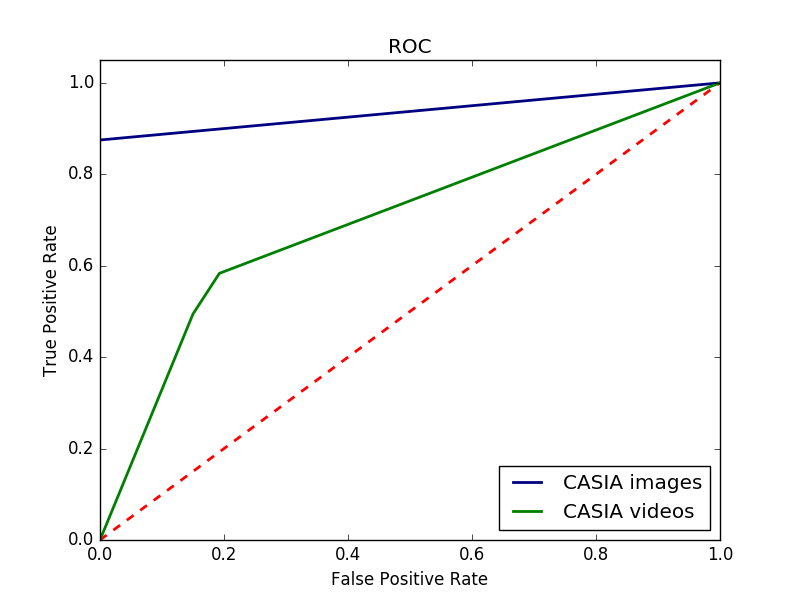
\includegraphics[width=0.58\textwidth]{images/comparative/CASIAs_KNN_ROC.png}
\caption{Comparative between CASIA databases with KNN classifier.} \label{fig:CASIAS_KNN_comparative}
\end{figure}

In figure \ref{fig:CASIAS_KNN_comparative} what is represented is the comparison between image CASIA (in blue) and video CASIA database (in green). As it can be seen, the result is much better when just CASIA images databases are used, although CASIA video results are not bad either.\\

\subsubsection{FRAVs databases}
Three FRAVs databases are compared in order to discuss if NIR images, in general, help to detect anti-spoofing attacks. In order to do so, and due to the large amount of data, one classifier is chosen to do the comparative: SVM with RBF kernel.\\

\begin{figure}[htb]
\centering
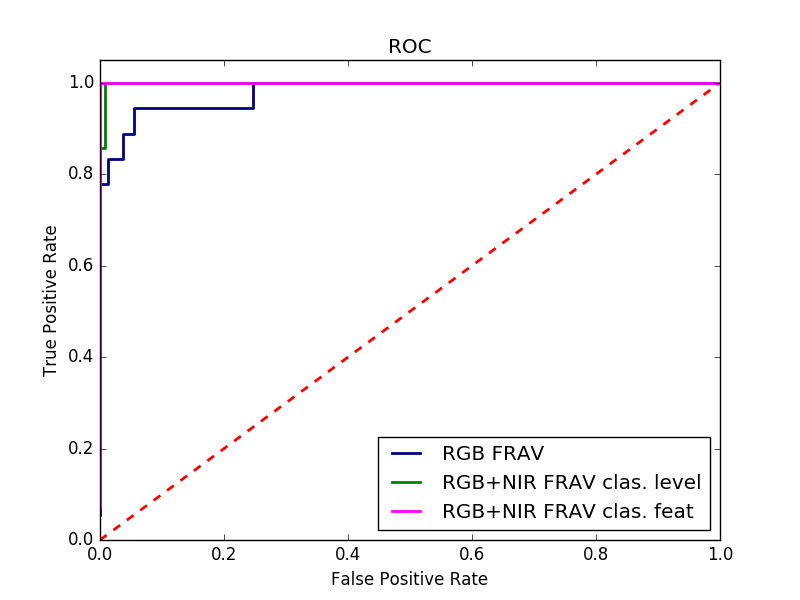
\includegraphics[width=0.58\textwidth]{images/comparative/FRAVs_SVM_RBF_ROC.png}
\caption{Comparative among FRAV databases with SVM RBF.} \label{fig:FRAVS_SVM_comparative}
\end{figure}

In figure \ref{fig:FRAVS_SVM_comparative} the three databases are represented: the RGB database in blue, the RGB+NIR FRAV database classification level in green and the RGB+NIR FRAV database  feature level in magenta. The ROC curve with NIR work better, in fact, it is almost perfect.\\

Figure \ref{fig:FRAVS_SVM_comparative}, along with the perfect APCR and the BPCR result obtained with logistic regression and the decision tree in the RGB+NIR feature level tends to conduce that NIR database improve the results.\\

\subsection{Results comparative with related works}\label{sec:comp_results_literature}
In order to compare results with related work, Equal Error rate (ERR) metric is going to be utilized. The comparative it is going to be made with CASIA database and MFSD-MSU database, because FRAV database results with others methods are not available.\\

In table \ref{table_literature_comp} are exposed EER(\%) of the results obtained with CASIA images database and CASIA video database with the literature review; In addition, the EER (\%) obtained with the proposed model is presented in the table with the literature review.\\

\begin{table}[]
\centering
\resizebox{\textwidth}{!}{%
\begin{tabular}{|c|c|cc}
\hline
\rowcolor[HTML]{ECF4FF}
\multicolumn{2}{|c|}{\cellcolor[HTML]{ECF4FF}\textbf{CASIA database}} & \multicolumn{2}{c|}{\cellcolor[HTML]{ECF4FF}\textbf{MFSD - MSU database}} \\ \hline
\rowcolor[HTML]{ECF4FF}
{\color[HTML]{333333} \textbf{CNN model}} & {\color[HTML]{333333} \textbf{EER (\%)}} & \multicolumn{1}{c|}{\cellcolor[HTML]{ECF4FF}\textbf{CNN model}} & \multicolumn{1}{c|}{\cellcolor[HTML]{ECF4FF}\textbf{EER (\%)}} \\ \hline
Own CASIA image  proposed model & 2.5 & \multicolumn{1}{c|}{Own MFSD-MSU proposed model} & \multicolumn{1}{c|}{5.4} \\ \hline
Own CASIA video proposed model & 11.5 & \multicolumn{1}{c|}{LDA+SVM proposed model in \cite{MSUdatabse}} & \multicolumn{1}{c|}{5.82} \\ \hline
CNN model proposed model in \cite{LSTM-CNN} & 6.2 &  &  \\ \cline{1-2}
LSTM-CNN proposed model in \cite{LSTM-CNN} & 5.17 &  &  \\ \cline{1-2}
CNN proposed model in \cite{yangLL14} & 4.64 &  &  \\ \cline{1-2}
LDA+SVM proposed model in \cite{MSUdatabse} & 12.9 &  &  \\ \cline{1-2}
\end{tabular}%
}
\caption{Comparative among proposed models and literature work.}
\label{table_literature_comp}
\end{table}

The researched work with MFSD-MSU is small and there is not researched work with Deep Learning.

\subsection{Executing time}
In this section, the time that has been necessary to carry out the training and testing processing described in this chapter are exposed.\\

Each general experiment is formed by the CNN training and the classification, which involves the search for the optimal parameter for each classifier, and the calculation of metrics. There are six general experiments, one per database used :
\begin{description}[itemsep=2pt,topsep=8pt,parsep=0pt,partopsep=20pt]
 \item Process 1: when CASIA image database has been used.
 \item Process 2: when CASIA video database has been used.
 \item Process 3: when RGB FRAV database has been used.
 \item Process 4: when RGB+NIR FRAV database (feature level) has been used.
 \item Process 5: when RGB+NIR FRAV database (classification level) has been used.
 \item Process 6: when MFSD database has been used.
\end{description}

In table \ref{table:Executing_time} the time (minutes) is exposed for each process. All the processes differ (generally) just in the database, so the differences in time is due to the fact that one database is bigger than other or because it is needed to train two different neural networks as in the RGB+NIR FRAV classification level.

\begin{table}[]
\centering
\begin{tabular}{|
>{\columncolor[HTML]{ECF4FF}}c |c|c|c|c|c|c|}
\hline
Process             & 1 & 2 & 3 & 4 & 5 & 6 \\ \hline
Executing Time(min) & 51.93  & 152.40  &  274.87 & 240.09  & 432.78  & 43.95
  \\ \hline
\end{tabular}
\caption{Executing time.}
\label{table:Executing_time}
\end{table}
